%% Преамбула TeX-файла

% 1. Стиль и язык
\documentclass[utf8x, 14pt]{G7-32} % Стиль (по умолчанию будет 14pt)
\usepackage{ragged2e}
\usepackage{microtype}


\justifying
\sloppy
\tolerance=500
\hyphenpenalty=10000
\emergencystretch=3em

% Остальные стандартные настройки убраны в preamble.inc.tex.
\sloppy

% Настройки стиля ГОСТ 7-32
% Для начала определяем, хотим мы или нет, чтобы рисунки и таблицы нумеровались в пределах раздела, или нам нужна сквозная нумерация.
\EqInChapter % формулы будут нумероваться в пределах раздела
\TableInChapter % таблицы будут нумероваться в пределах раздела
\PicInChapter % рисунки будут нумероваться в пределах раздела

% Добавляем гипертекстовое оглавление в PDF
\usepackage[
bookmarks=true, colorlinks=true, unicode=true,
urlcolor=black,linkcolor=black, anchorcolor=black,
citecolor=black, menucolor=black, filecolor=black,
]{hyperref}
% Изменение начертания шрифта --- после чего выглядит таймсоподобно.
% apt-get install scalable-cyrfonts-tex

\IfFileExists{cyrtimes.sty}
    {
        \usepackage{cyrtimespatched}
    }
    {
        % А если Times нету, то будет CM...
    }

\usepackage{graphicx}   % Пакет для включения рисунков

% С такими оно полями оно работает по-умолчанию:
%\RequirePackage[left=30mm,right=10mm,top=20mm,bottom=20mm,headsep=0pt]{geometry}
% Если вас тошнит от поля в 10мм --- увеличивайте до 20-ти, ну и про переплёт не забывайте:
%\geometry{right=10mm}
%\geometry{left=30mm}


% Пакет Tikz
\usepackage{tikz}
\usetikzlibrary{arrows,positioning,shadows}

% Произвольная нумерация списков.
\usepackage{enumerate}

% ячейки в несколько строчек
\usepackage{multirow}

% itemize внутри tabular
\usepackage{paralist,array}

% псевдокод
\usepackage{algorithm2e}

\SetKwInput{KwData}{Исходные параметры}
\SetKwInput{KwResult}{Результат}
\SetKwInput{KwIn}{Входные данные}
\SetKwInput{KwOut}{Выходные данные}
\SetKwIF{If}{ElseIf}{Else}{если}{тогда}{иначе если}{иначе}{конец условия}
\SetKwFor{While}{пока}{выполнять}{конец цикла}
\SetKw{KwTo}{от}
\SetKw{KwRet}{возвратить}
\SetKw{Return}{возвратить}
\SetKwBlock{Begin}{начало блока}{конец блока}
\SetKwSwitch{Switch}{Case}{Other}{Проверить значение}{и выполнить}{вариант}{в противном случае}{конец варианта}{конец проверки значений}
\SetKwFor{For}{цикл}{выполнять}{конец цикла}
\SetKwFor{ForEach}{для каждого}{выполнять}{конец цикла}
\SetKwRepeat{Repeat}{повторять}{до тех пор, пока}
\SetAlgorithmName{Алгоритм}{алгоритм}{Список алгоритмов}


% Настройки листингов.
\ifPDFTeX
% 8 Листинги

\usepackage{listings}
% Значения по умолчанию
\lstset{
  basicstyle= \footnotesize,
  breakatwhitespace=true,% разрыв строк только на whitespacce
  breaklines=true,       % переносить длинные строки
%   captionpos=b,          % подписи снизу -- вроде не надо
  inputencoding=koi8-r,
  numbers=left,          % нумерация слева
  numberstyle=\footnotesize,
  showspaces=false,      % показывать пробелы подчеркиваниями -- идиотизм 70-х годов
  showstringspaces=false,
  showtabs=false,        % и табы тоже
  stepnumber=1,
  tabsize=4,              % кому нужны табы по 8 символов?
  frame=single
}

% Стиль для псевдокода: строчки обычно короткие, поэтому размер шрифта побольше
\lstdefinestyle{pseudocode}{
  basicstyle=\small,
  keywordstyle=\color{black}\bfseries\underbar,
  language=Pseudocode,
  numberstyle=\footnotesize,
  commentstyle=\footnotesize\it
}

% Стиль для обычного кода: маленький шрифт
\lstdefinestyle{realcode}{
  basicstyle=\scriptsize,
  numberstyle=\footnotesize
}

% Стиль для коротких кусков обычного кода: средний шрифт
\lstdefinestyle{simplecode}{
  basicstyle=\footnotesize,
  numberstyle=\footnotesize
}

% Стиль для BNF
\lstdefinestyle{grammar}{
  basicstyle=\footnotesize,
  numberstyle=\footnotesize,
  stringstyle=\bfseries\ttfamily,
  language=BNF
}

% Определим свой язык для написания псевдокодов на основе Python
\lstdefinelanguage[]{Pseudocode}[]{Python}{
  morekeywords={each,empty,wait,do},% ключевые слова добавлять сюда
  morecomment=[s]{\{}{\}},% комменты {а-ля Pascal} смотрятся нагляднее
  literate=% а сюда добавлять операторы, которые хотите отображать как мат. символы
    {->}{\ensuremath{$\rightarrow$}~}2%
    {<-}{\ensuremath{$\leftarrow$}~}2%
    {:=}{\ensuremath{$\leftarrow$}~}2%
    {<--}{\ensuremath{$\Longleftarrow$}~}2%
}[keywords,comments]

% Свой язык для задания грамматик в BNF
\lstdefinelanguage[]{BNF}[]{}{
  morekeywords={},
  morecomment=[s]{@}{@},
  morestring=[b]",%
  literate=%
    {->}{\ensuremath{$\rightarrow$}~}2%
    {*}{\ensuremath{$^*$}~}2%
    {+}{\ensuremath{$^+$}~}2%
    {|}{\ensuremath{$|$}~}2%
}[keywords,comments,strings]

% Подписи к листингам на русском языке.
\renewcommand\lstlistingname{\cyr\CYRL\cyri\cyrs\cyrt\cyri\cyrn\cyrg}
\renewcommand\lstlistlistingname{\cyr\CYRL\cyri\cyrs\cyrt\cyri\cyrn\cyrg\cyri}

\else
\usepackage{local-minted}
\fi

\usepackage{pdfpages}

% Полезные макросы листингов.
% Любимые команды
\newcommand{\Code}[1]{\textbf{#1}}


\begin{document}


\includepdf[pages=-]{title.pdf}

\frontmatter % выключает нумерацию ВСЕГО; здесь начинаются ненумерованные главы: реферат, введение, глоссарий, сокращения и прочее.

тз
\newpage
тз
\newpage
план
\newpage

% Команды \breakingbeforechapters и \nonbreakingbeforechapters
% управляют разрывом страницы перед главами.
% По-умолчанию страница разрывается.

% \nobreakingbeforechapters
% \breakingbeforechapters

% Также можно использовать \Referat, как в оригинале
\Referat
%\begin{abstract}
Дипломная работа: 64 страницы, 24 рисунка, 8 таблиц, 30 источников.

В магистерской диссертации рассмотрена задача распознавания статических жестов. Проведен анализ предметной области, проанализированы известные методы решения данной задачи и обоснована необходимость построения метода, объединяющего преимущества существующих подходов. Разработан метод распознавания, основанны на использовании искусственных нейронных сетей, модифицированный путем добавления предобработки изображений с целью упрощения процесса классификации и использования в качестве классификатора капсульный нейронных сетей. Разработаны алгоритмические структуры для реализации комбинированного метода. Осуществлена программная реализация предложенного решения. Прове­дены вычислительные исследования, подтверждающие работоспособ­ность метода и показывающие точность распознавания свыше 95\%.

Результаты исследовательской деятельности были отражены в печатной работе.

В первом разделе приводится сравнительный анализ известных методов распознавания жестовых символов, на основании которого выбран прототип, для которого будут проводится исследования. Обоснована необходимость построение нового метода. Во втором разделе описан метод распознавания жестовых символов, описаны структуры, необходимые для его реализации. В третьем разделе описана архитектура программной реализации предложенного метода, обоснован выбор средств программной реализации. Описаны ресурсы, необходимые для сборки и запуска разработанного программного обеспечения, форматы входных и выходных файлов, а также интерфейс и руководство пользователя. В четвертом разделе описаны и проведены вычислительные экспери­ менты для исследования предложенного метода.

%\end{abstract}

%%% Local Variables: 
%%% mode: latex
%%% TeX-master: "rpz"
%%% End: 


\tableofcontents

\Defines % Необходимые определения. Вряд ли понадобться
В настоящей работе используются следующие термины с соответствующими определениями.
\begin{description}
	\item [Жест] осознанное движение человеческого тела или его части, которое несет информацию и совершается с целью её передачи.
	\item[Капсула] группа искусственных нейровон, инкапсулирующая в себе информацию в векторном виде.
	\item[Скелет] множество точек, равноудаленных от границы области.
%\item[Дискретизация] преобразование непрерывного информационного множества аналоговых сигналов в дискретное множество.
%\item[Музыкальное произведение] последовательность сочетаний звуков.
%\item[Звук] физическое явление, представляющее собой распространение в виде упругих волн механических колебаний в твёрдой, жидкой или газообразной среде.
%\item[Колебания] повторяющийся в той или иной степени во времени процесс изменения состояний системы около точки равновесия. Колебания характеризуются частотой, фазой и амплитудой.
%\item[Частота] физическая величина, характеристика периодического процесса, равна количеству повторений или возникновения событий в единицу времени. Единица измерения -- герцы (Гц).
%\item[Фаза] аргумент периодической функции, описывающей колебательный или волновой процесс.
%\item[Амплитуда] максимальное значение смещения или изменения перемен­ ной величины от среднего значения при колебательном или волновом движении.
%Применительно к музыке вместо общего термина <<звук>> используют более конкретный термин <<музыкальный звук>>.
%\item[Музыкальный звук] это звук определённой высоты, использующийся
%как материал для создания музыкальных сочинений. Для письменной фиксации му­зыкальных звуков используется нотация. Наиболее распространённые формы записи высотных значений музыкальных звуков – латинская буквенная (C, D, E, F, G, A, B/H) или слоговая (до, ре, ми, фа, соль, ля, си) нотация. В данной работе для обозначения музыкальных звуков используется латинская буквенная нотация с указанием номера октавы.
%\item[Нота] музыкальный звук или его письменная запись.

%Далее понятие <<звук>> используется в смысле музыкального звука.

%\item[Аккомпанемент] сопровождение одним или несколькими инструментами, а также оркестром сольной партии (певца, инструменталиста, хора и других). Сопроводителя называют аккомпаниатором. Аккомпанементом также называют гармоническое и ритмическое сопровождение основной мелодии, голоса.
%\item[Вокал (или пение)] исполнение мелодии с помощью голоса человека.
%\item[Тембр] (обертоновая) окраска звука, <<качество тона>>.
%\item[Рефакторинг] процесс изменения внутренней структуры программы, не затрагивающий её внешнего поведения и имеющий целью облегчить понимание её работы.
%\item[Цифровая звуковая рабочая станция] электронная или компьютерная система, предназначенная для записи, хранения, редактирования и воспроизведения цифрового звука. Предусматривает возможность выполнения на ней законченного цикла работ, от первичной записи до получения готового результата.
\end{description}

%%% Local Variables:
%%% mode: latex
%%% TeX-master: "rpz"
%%% End:

\Abbreviations %% Список обозначений и сокращений в тексте
\begin{description}
\item[СММ] Скрытая марковская модель
\item[ASL] American Sign Language
\item[СКК] Самоорганизующаяся карта Кохонена
\item[СНС] Сверточные нейронные сети
\item[КНС] Капсульные нейронные сети
\end{description}

%%% Local Variables:
%%% mode: latex
%%% TeX-master: "rpz"
%%% End:


\Introduction

Одной из актуальных задач в области компьютерного зрения является распознавание жестов. Качественный метод распознавания жестов позволит дать развитие многим системам, например интеллектуальные жестовые интерфейсы, системы перевода с жестовых языков, управление для систем виртуальной и дополненной реальностей. В настоящее время известен ряд практически применимых решений данной задачи \cite{Suharjito}, но все они имеют недостатки, например необходимость использования дополнительных источников данных (перчатки с датчиками).

Целью даной работы является разработка метода распознавания жестовых символов. Для решения поставленной задачи необходимо:

\begin{itemize}
	\item проанализировать предметную область;
	\item проанализировать существующие методы распознавания жестов;
	\item на основе полученных во время анализа данных разработать собственный метод распознавания жестовых символов;
	\item реализовать разработанный метод в программном продукте;
	\item провести планирование и постановку экспериментов с целью выяснения качества работы разработанного метода.
\end{itemize}

\mainmatter % это включает нумерацию глав и секций в документе ниже

\chapter{Аналитический раздел}
\label{cha:analysis}

Известные на данный момент методы распознавания жестовых символов, как правило, реализуют три этапа обработки информации:

\begin{enumerate}
	\item получение данных о жесте;
	\item предобработка данных;
	\item классификация жестов.
\end{enumerate}

В качестве входных данных можно использовать кинематические трехмерные модели рук, получаемых с помощью специальных устройств ввода, таких как Microsoft Kinect\cite{Wang} и Leap Motion Controller\cite{Mohandes}. Такие методы обеспечивают достаточно высокую точность распознавания, позволяя обнаруживать различные жесты, но при этом требуют большого объема вычислений и наличия обширной базы данных, содержащей все жесты. Так же данные методы получения информации о жесте требуют наличия дополнительных устройств ввода. Из-за этого, данную группу способов получения информации о жестах решено не рассматривать в данной работе.

В качестве другого источника данных можно использовать RGB изображения, полученные, например, с web-камеры ПК или камеры смартфона. Преимуществом данного подхода является распространенность данных устройств ввода. Web-камерой в наше время оснащен каждый ноутбук, а смартфонами владеет 45\% населения Земли \cite{smartfones}.

\section{Алгоритмы предобработки изображения кисти руки, применимых к распознаванию жестовых символов}

Скорость и качество работы алгоритмов классификации во многом зависит от исходных данных. Например, для классификации жестов с помощью скрытой марковской модели\cite{Zhang} основные признаки получаются из изображения рук в разноцветных перчатках. Тем самым, важно подобрать метод предобработки изображения таким образом, чтобы его применение в итоговом методе упрощало процесс классификации, не увеличивая при этом общее время работы. Известные алгоритмы, применимые для достижения данной цели, можно разделить на следующие группы:

\begin{itemize}
	\item выделение контура фигуры;
	\item выделение силуэта кисти руки;
	\item построение скелета кисти руки.
\end{itemize}

Рассмотрим каждую из этих групп.

\subsection{Выделение контура фигуры}

Для выделения контура кисти руки можно использовать детекторы границ, определяющие градиент яркости черно-белого изображения. Поэтому предварительным этапом данных методов является преобразование изображения из цветного в черно-белое. К вышеуказанным методам относят:

\begin{itemize}
	\item оператор Собеля\cite{Sobel};
	\item оператор Прюитт\cite{Prewitt};
	\item перекрестный оператор Робертса\cite{Roberts};
	\item оператор Кэнни\cite{Canny}.
\end{itemize}

\section*{Операторы Собеля, Прюитт и Робертса}

Принцип работы данных алгоритмов \cite{Sobel,Prewitt,Roberts} заключается в свертке изображения двумя сепарабельными целочисленными фильтрами. Общая схема работы методов представлена на рис. \ref{an:sobel}.

\begin{figure}[!h]
	\centering
	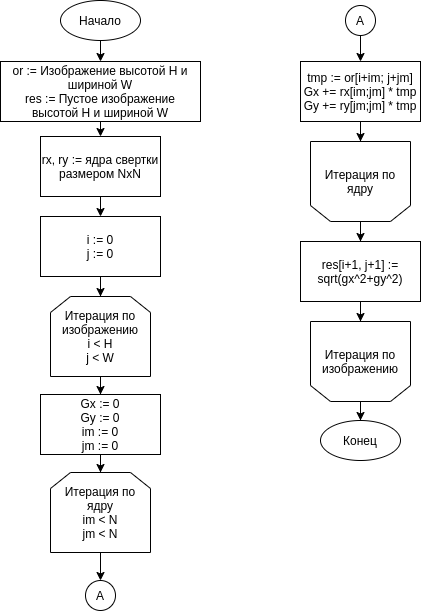
\includegraphics[width=0.6\textwidth]{inc/img/sobel_block}
	\caption{Общая схема алгоритмов определения границ изображения}
	\label{an:sobel}
\end{figure}

Разница алгоритмов заключается в способе задания ядер свертки:

Оператор Собеля:

\begin{eqnarray}\label{eq:sobel-matrixs}
G_x = \begin{bmatrix}
-1 & 0 & 1\\
-2 & 0 & 2\\
-1 & 0 & 1\\
\end{bmatrix} 
G_y = \begin{bmatrix}
-1 & -2 & -1\\
0 & 0 & 0\\
1 & 2 & 1\\
\end{bmatrix}
\end{eqnarray}

Оператор Прюитт:

\begin{eqnarray}\label{eq:prewitt-matrixs}
G_x = \begin{bmatrix}
-1 & 0 & 1\\
-1 & 0 & 1\\
-1 & 0 & 1\\
\end{bmatrix} 
G_y = \begin{bmatrix}
-1 & -1 & -1\\
0 & 0 & 0\\
1 & 1 & 1\\
\end{bmatrix}
\end{eqnarray}

Из-за меньшего значения средних элементов итоговое изображение имеет более явный эффект сглаживания.

Перекрестный оператор Робертса:

\begin{eqnarray}\label{eq:roberts-matrixs}
G_x = \begin{bmatrix}
1 & 0\\
0 & -1
\end{bmatrix} 
G_y = \begin{bmatrix}
0 & 1\\
-1 & 0
\end{bmatrix}
\end{eqnarray}

Недостатком данного метода является отсутствие четко выраженного центрального элемента у ядра свертки. Но эта особенность алгоритма обуславливает высокую скорость обработки изображения.

В итоговом изображении в каждый пиксель записывается значение изменения яркости пикселя исходного изображения относительно соседних, вычисляемое по формуле $G=\sqrt{G_x^2+G_y^2}$, т. е. чем выше итоговое число, тем вероятнее, что данный пиксель находится на границе.

\section*{Оператор Кэнни}

Метод\cite{Canny} был разработан с целью удовлетворения следующим условиям:

\begin{itemize}
	\item хорошее обнаружение (Кэнни трактовал это свойство как повышение отношения сигнал/шум);
	\item хорошая локализация (правильное определение положения границы);
	\item единственный отклик на одну границу.
\end{itemize}

Схема работы алгоритма представлена на рис. \ref{an:canny}. Рассмотрим каждый этап подробнее с наглядной визуализацией обработки. Для этого применим данный оператор шаг за шагом к изображению, приведенному на рис. \ref{fig:canny}a.

\begin{figure}[!h]
	\centering
	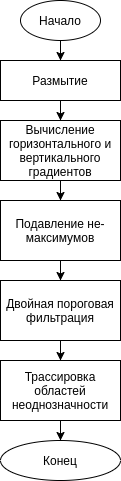
\includegraphics[width=0.15\textwidth]{inc/img/canny-block}
	\caption{Схема алгоритма оператора Кэнни}
	\label{an:canny}
\end{figure}

\begin{figure}[ht!]
	\begin{minipage}[h]{0.49\linewidth}
		\center{
\includegraphics[width=0.5\linewidth]{inc/img/bmstu_gray} \\ а)}
	\end{minipage}
	\hfill
	\begin{minipage}[h]{0.49\linewidth}
		\center{
\includegraphics[width=0.5\linewidth]{inc/img/bmstu_smoothed} \\ б)}
	\end{minipage}
	\begin{minipage}[h]{0.49\linewidth}
		\center{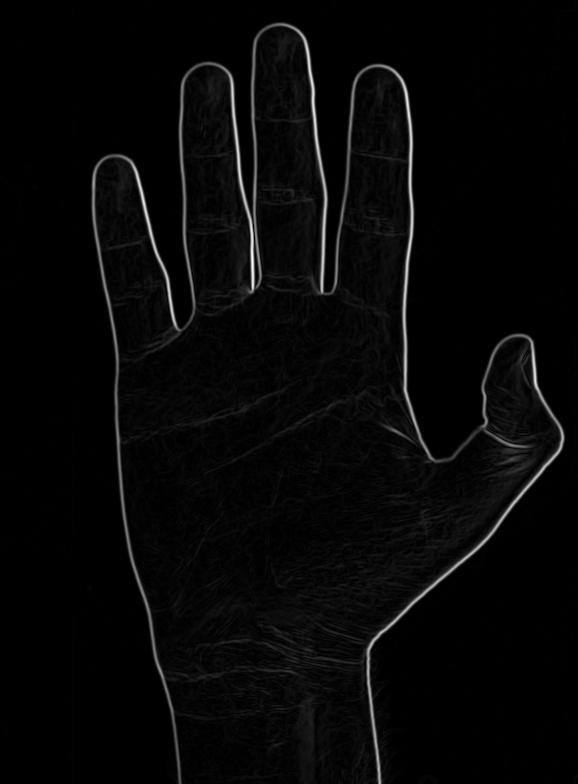
\includegraphics[width=0.5\linewidth]{inc/img/bmstu_gradient} \\ в)}
	\end{minipage}
	\hfill
	\begin{minipage}[h]{0.49\linewidth}
		\center{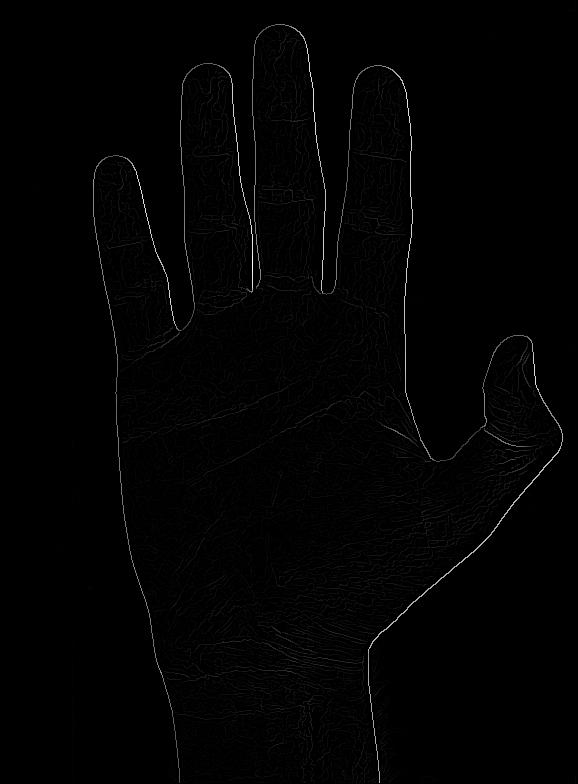
\includegraphics[width=0.5\linewidth]{inc/img/bmstu_non_max} \\ г)}
	\end{minipage}
	\begin{minipage}[h]{0.49\linewidth}
		\center{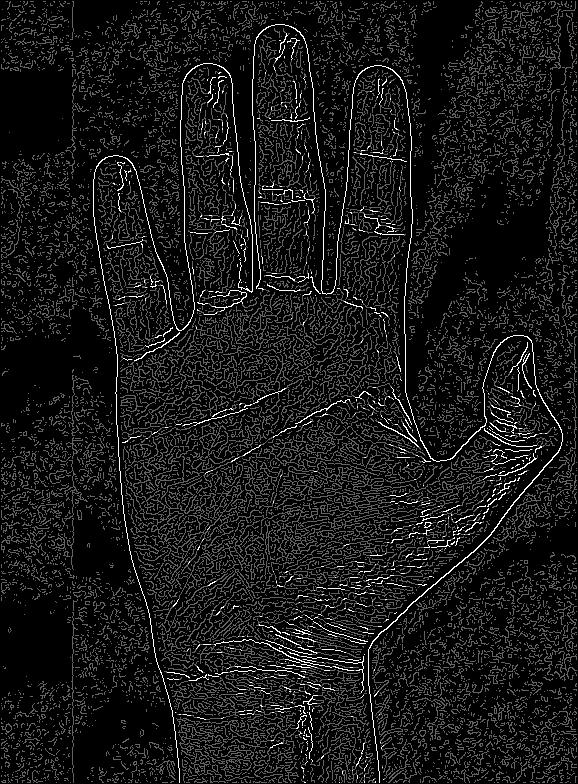
\includegraphics[width=0.5\linewidth]{inc/img/bmstu_threshold} \\ д)}
	\end{minipage}
	\hfill
	\begin{minipage}[h]{0.49\linewidth}
		\center{
\includegraphics[width=0.5\linewidth]{inc/img/bmstu_final} \\ е)}
	\end{minipage}
	\caption{Результаты экспериментального исследования этапов оператора Кэнни: а) исходное изображение; б) применение размытия; в) поиск градиентов; г) подавление	не-максимумов; д) двойная пороговая фильтрация; е) трассировка областей неоднозначности}
	\label{fig:canny}
\end{figure}

\begin{enumerate}
	\item Размытие изображения. Данный этап, как видно на рис. \ref{fig:canny}б, необходим для устранения лишних шумов, способных понизить качество последующих	этапов выделения границ.
	\item Поиск градиентов яркости. На данном этапе был применен оператор Собеля, описанный ранее. В результате на рис. \ref{fig:canny}в были получены точки, наиболее вероятно находящиеся на границах изображения\cite{Suharjito}.
	\item Подавление <<не-максимумов>>. Как видно на рис. \ref{fig:canny}г, на данном этапе отбрасываются точки, значение градиента которых не является локальным максимумом, т. е. такие точки являются ложными границами.
	\item Определение потенциальных границ с помощью двойной пороговой фильтрации. При этом используется два порога фильтрации:
	\begin{itemize}
		\item Все пиксели со значением больше верхней границы принимают максимальное значение (достоверная граница).
		\item Все пиксели со значением меньше нижней границы подавляются.
		\item Все пиксели со значением в диапазоне границ принимают фиксированное среднее значение. Их уточнение происходит на следующем этапе.
	\end{itemize}
	На рис. \ref{fig:canny}д представлен результат применения данной фильтрации с порогами 0.03 и 0.07. В результирующую достоверную границу была добавлена часть контура тени кисти.
	\item Трассировка области неоднозначности. После данного этапа, как видно на рис. \ref{fig:canny}е были отброшены все неопределенные границы, потому что они не были связаны с уже определенной границей.
\end{enumerate}

\subsection{Выделение силуэта кисти руки}
\label{cha:syl}
Помимо классических методов определения границ, можно использовать сегментацию по цвету кожи\cite{Phung}. Данный метод преобразует RGB изображение в бинарное с помощью фильтрации пикселей по цвету, близкому к цвету кожи. Для улучшения работы алгоритма перед фильтрацией изображение переводят в цветовое пространство YCrCb, в котором различные цвета кожи расположены близко друг к другу\cite{Siddharth}.

Как правило, после бинаризации на изображении присутствуют шумы и артефакты, вызванные тем, что на фоновой части изображения находились пиксели,
попадающие в ограничения фильтра. Для их устранения можно использовать морфологические операции: «наращивание» и «эрозия»\cite{DIP}.

Пусть имеется бинарное изображение A и структурный элемент B c началом координат в его центре (рис. \ref{an:morph}).

\begin{figure}[!h]
	\centering
	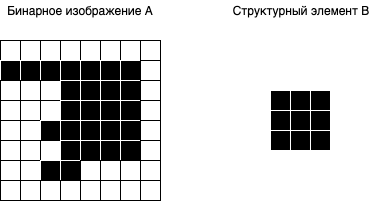
\includegraphics[width=0.6\textwidth]{inc/img/morf}
	\caption{Бинарное изображение и структурный элемент}
	\label{an:morph}
\end{figure}

Наращивание. Каждый раз, когда начало координат структурного элемента совмещается с единичным бинарным пикселем, ко всему структурному элементу применяется перенос и последующее логическое сложение с соответствующими пикселями бинарного изображения (рис. \ref{an:dil}).

\begin{figure}[!h]
	\centering
	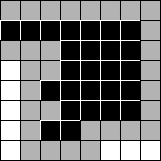
\includegraphics[width=0.3\textwidth]{inc/img/dil}
	\caption{Наращивание бинарного изображения A структурным элементом B}
	\label{an:dil}
\end{figure}

Эрозия. Если в некоторой позиции каждый единичный пиксель структурного элемента совпадает с единичным пикселем бинарного изображения, то выполняется логическое сложение центрального пикселя структурного элемента с соответствующим пикселем выходного изображения (рис. \ref{an:eros}).

\begin{figure}[!h]
	\centering
	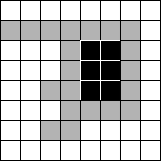
\includegraphics[width=0.3\textwidth]{inc/img/eros}
	\caption{Эрозия бинарного изображения A структурным элементом B}
	\label{an:eros}
\end{figure}

\subsection{Построение скелета кисти руки}

Для ускорения процесса классификации жеста руки можно использовать скелетную модель. Данный тип входных данных в силу своей специфики может упростить вычисление признаков, необходимых классификатору.

Для построения скелета кисти можно использовать метод построения скелета выпуклой фигуры\cite{DIP}.

В качестве выпуклой фигуры можно использовать результат работы метода выделения силуэта кисти руки, описанного в разделе \ref{cha:syl}.

В данном методе предлагается последовательное применение морфологической операции «эрозия» (рис. \ref{an:eros}) до тех пор, пока результатом следующей итерации не станет пустое изображение.

Недостатком данного метода являются побочные ветви скелета, образованные из-за возможной зашумленности или неточности фигуры. Другим недостатком можно считать высокую вероятность получения несвязного набора пикселей для всего скелета или обеспечения одинаковой ширины ветвей во всем скелете.

Для решения данных проблем можно обратиться к технологиям машинного обучения. Скелет кисти можно построить на основании ключевых точек, получаемых с помощью нейронной сети\cite{DNN}. Данная нейронная сеть определяет на изображении 22 ключевые точки, 21 из которых относится к кисти руки, а 22 — отмечают фон. Пример расположения точек представлен на рис. \ref{an:handpose}.

\begin{figure}[!h]
	\centering
	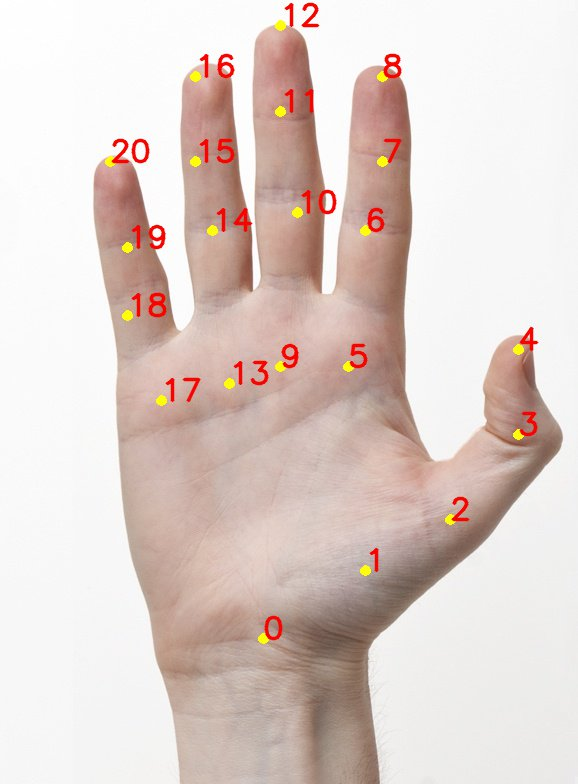
\includegraphics[width=0.3\textwidth]{inc/img/handpose-demo-keypoints}
	\caption{Ключевые точки кисти руки}
	\label{an:handpose}
\end{figure}

Далее для построения скелета необходимо соединить полученные точки в последовательностях, описанной в табл. \ref{an:poses-table}.

\begin{table}[h]
	\caption{\label{an:poses-table}Последовательность соединения ключевых точек}
	\begin{center}
		\begin{tabular}{|p{0.45\textwidth}|p{0.45\textwidth}|}
			\hline
			Ветвь скелета & Последовательность точек \\
			\hline
			Большой палец & 0$\rightarrow$1$\rightarrow$2$\rightarrow$3$\rightarrow$4 \\	
			\hline
			Указательный палец & 0$\rightarrow$5$\rightarrow$6$\rightarrow$7$\rightarrow$8\\	
			\hline
			Средний палец & 0$\rightarrow$9$\rightarrow$10$\rightarrow$11$\rightarrow$12 \\
			\hline
			Безымянный палец & 0$\rightarrow$13$\rightarrow$14$\rightarrow$15$\rightarrow$16 \\
			\hline
			Мизинец & 0$\rightarrow$17$\rightarrow$18$\rightarrow$19$\rightarrow$20 \\
			\hline
		\end{tabular}
	\end{center}
\end{table}

\subsection{Сравнение алгоритмов предобработки изображений}

Сравнительный анализ описанных выше методов был проведен в работе \cite{Tantsevov}. Каждый из алгоритмов был применен для обработки одинакового набора данных, состоящего из растровых изображений кистей рук; тестовая выборка составлялась из наборов данных, различающихся форматами изображений, их размерами и физиологическими особенностями кистей рук. Все данные находятся в открытом доступе:

\begin{itemize}
	\item ASL Alphabet. Image data set for alphabets in the American Sign Language;
	\item Hand Gesture of the Colombian sign language. Hand gestures, recognizing the numbers from 0 to 5 and the vowels;
	\item ASL Fingerspelling Images (RGB \& Depth);
	\item <<sign language between 0 9>>.
\end{itemize}

Замеры времени обработки каждого изображения для получения статистики проводились по минимальному, максимальному и среднему времени работы алгоритма. Результаты экспериментов представлены для каждого набора данных: для ASL Alphabet представлены в табл. \ref{tab:asl-alphaber}; для Hand Gesture of the Colombian sign language -- в табл. \ref{tab:colombian-alphaber}; для ASL Fingerspelling Images — в табл. \ref{tab:asl2-alphaber}; для <<sign language between 0 9>> — в табл. \ref{tab:datamix-alphaber}.

\begin{table}[h]
	\caption{\label{tab:asl-alphaber}Время работы алгоритмов (в секундах) на наборе данных ASL Alphabet}
	\begin{center}
		\begin{tabular}{|p{0.38\textwidth}|p{0.18\textwidth}|p{0.18\textwidth}|p{0.14\textwidth}|}
			\hline
			Название алгоритма & Минимальное время & Максимальное время & Среднее время \\
			\hline
			Оператор Кэнни & 0.1783 & 0.4642 & 0.2553 \\
			Оператор Робертса & 0.0687 & 0.1252 & 0.0852 \\
			Оператор Прюитт & 0.1175 & 0.2211 & 0.1424  \\
			Оператор Собеля & 0.1177 & 0.3112 & 0.1527 \\
			Выделение силуэта & 0.0668 & 0.2101 & 0.0901 \\
			Морфологическое построение скелета & 0.2084 & 1.2112 & 0.3068 \\
			Построение скелета по ключевым точкам & 1.408 & 3.4571 & 2.042 \\
			\hline
		\end{tabular}
	\end{center}
\end{table}

\begin{table}[h]
	\caption{\label{tab:colombian-alphaber}Время работы алгоритмов (в секундах) на наборе данных Hand Gesture of the Colombian sign language}
	\begin{center}
		\begin{tabular}{|p{0.38\textwidth}|p{0.18\textwidth}|p{0.18\textwidth}|p{0.14\textwidth}|}
			\hline
			Название алгоритма & Минимальное время & Максимальное время & Среднее время \\
			\hline
			Оператор Кэнни & 53.5126 & 72.6076 & 62.971 \\
			Оператор Робертса & 22.2837 & 54.2706 & 25.8842 \\
			Оператор Прюитт & 38.7491 & 99.2961 & 46.5944 \\
			Оператор Собеля & 38.8739 & 104.1867 & 46.9016 \\
			Выделение силуэта & 22.3001 & 32.8930 & 23.5992 \\
			Морфологическое построение скелета & 65.3335 & 88.3565 & 69.0014 \\
			Построение скелета  по ключевым точкам & 3.0844 & 4.2156 & 3.2775 \\
			\hline
		\end{tabular}
	\end{center}
\end{table} 

\begin{table}[!h]
	\caption{\label{tab:asl2-alphaber}Время работы алгоритмов (в секундах) на наборе данных ASL Fingerspelling Images}
	\begin{center}
		\begin{tabular}{|p{0.38\textwidth}|p{0.18\textwidth}|p{0.18\textwidth}|p{0.14\textwidth}|}
			\hline
			Название алгоритма & Минимальное время & Максимальное время & Среднее время \\
			\hline
			Оператор Кэнни & 0.0193 & 0.0816 & 0.0545 \\
			Оператор Робертса & 0.0111 & 0.0476 & 0.0286 \\
			Оператор Прюитт & 0.0179 & 0.0864 & 0.0495 \\
			Оператор Собеля & 0.0217 & 0.0847 & 0.0469 \\
			Выделение силуэта & 0.0114 & 0.0506 & 0.0277 \\
			Морфологическое построение скелета & 0.0343 & 0.1852 & 0.0884 \\
			Построение скелета по ключевым точкам & 0.6251 & 3.3092 & 1.5665 \\
			\hline
		\end{tabular}
	\end{center}
\end{table}

\begin{table}[!h]
	\caption{\label{tab:datamix-alphaber}Время работы алгоритмов (в секундах) на наборе данных sign language between 0 9}
	\begin{center}
		\begin{tabular}{|p{0.38\textwidth}|p{0.18\textwidth}|p{0.18\textwidth}|p{0.14\textwidth}|}
			\hline
			Название алгоритма & Минимальное время & Максимальное время & Среднее время \\
			\hline
			Оператор Кэнни & 0.333 & 0.7686 & 0.4708 \\
			Оператор Робертса & 0.1566 & 0.246 & 0.1778 \\
			Оператор Прюитт & 0.271 & 0.3751 & 0.3027 \\
			Оператор Собеля & 0.2718 & 0.655 & 0.3295 \\
			Выделение силуэта & 0.1486 & 0.4709 & 0.2085 \\
			Морфологическое построение скелета & 0.4471 & 1.637 & 0.6518 \\
			Построение скелета по ключевым точкам & 1.4346 & 3.2976 & 2.0723 \\
			\hline
		\end{tabular}
	\end{center}
\end{table}

Метод выделения силуэта показал наилучшие временные результаты (табл. \ref{tab:asl-alphaber}). Также при правильной предварительной настройке метода можно добиться удовлетворительной четкости выделения. Тем не менее предварительная настройка является главной проблемой этого алгоритма. На рис. \ref{an:compare} видно, что при неудачном выборе начальных настроек алгоритм не справляется со своей задачей.

\begin{figure}[!h]
	\centering
	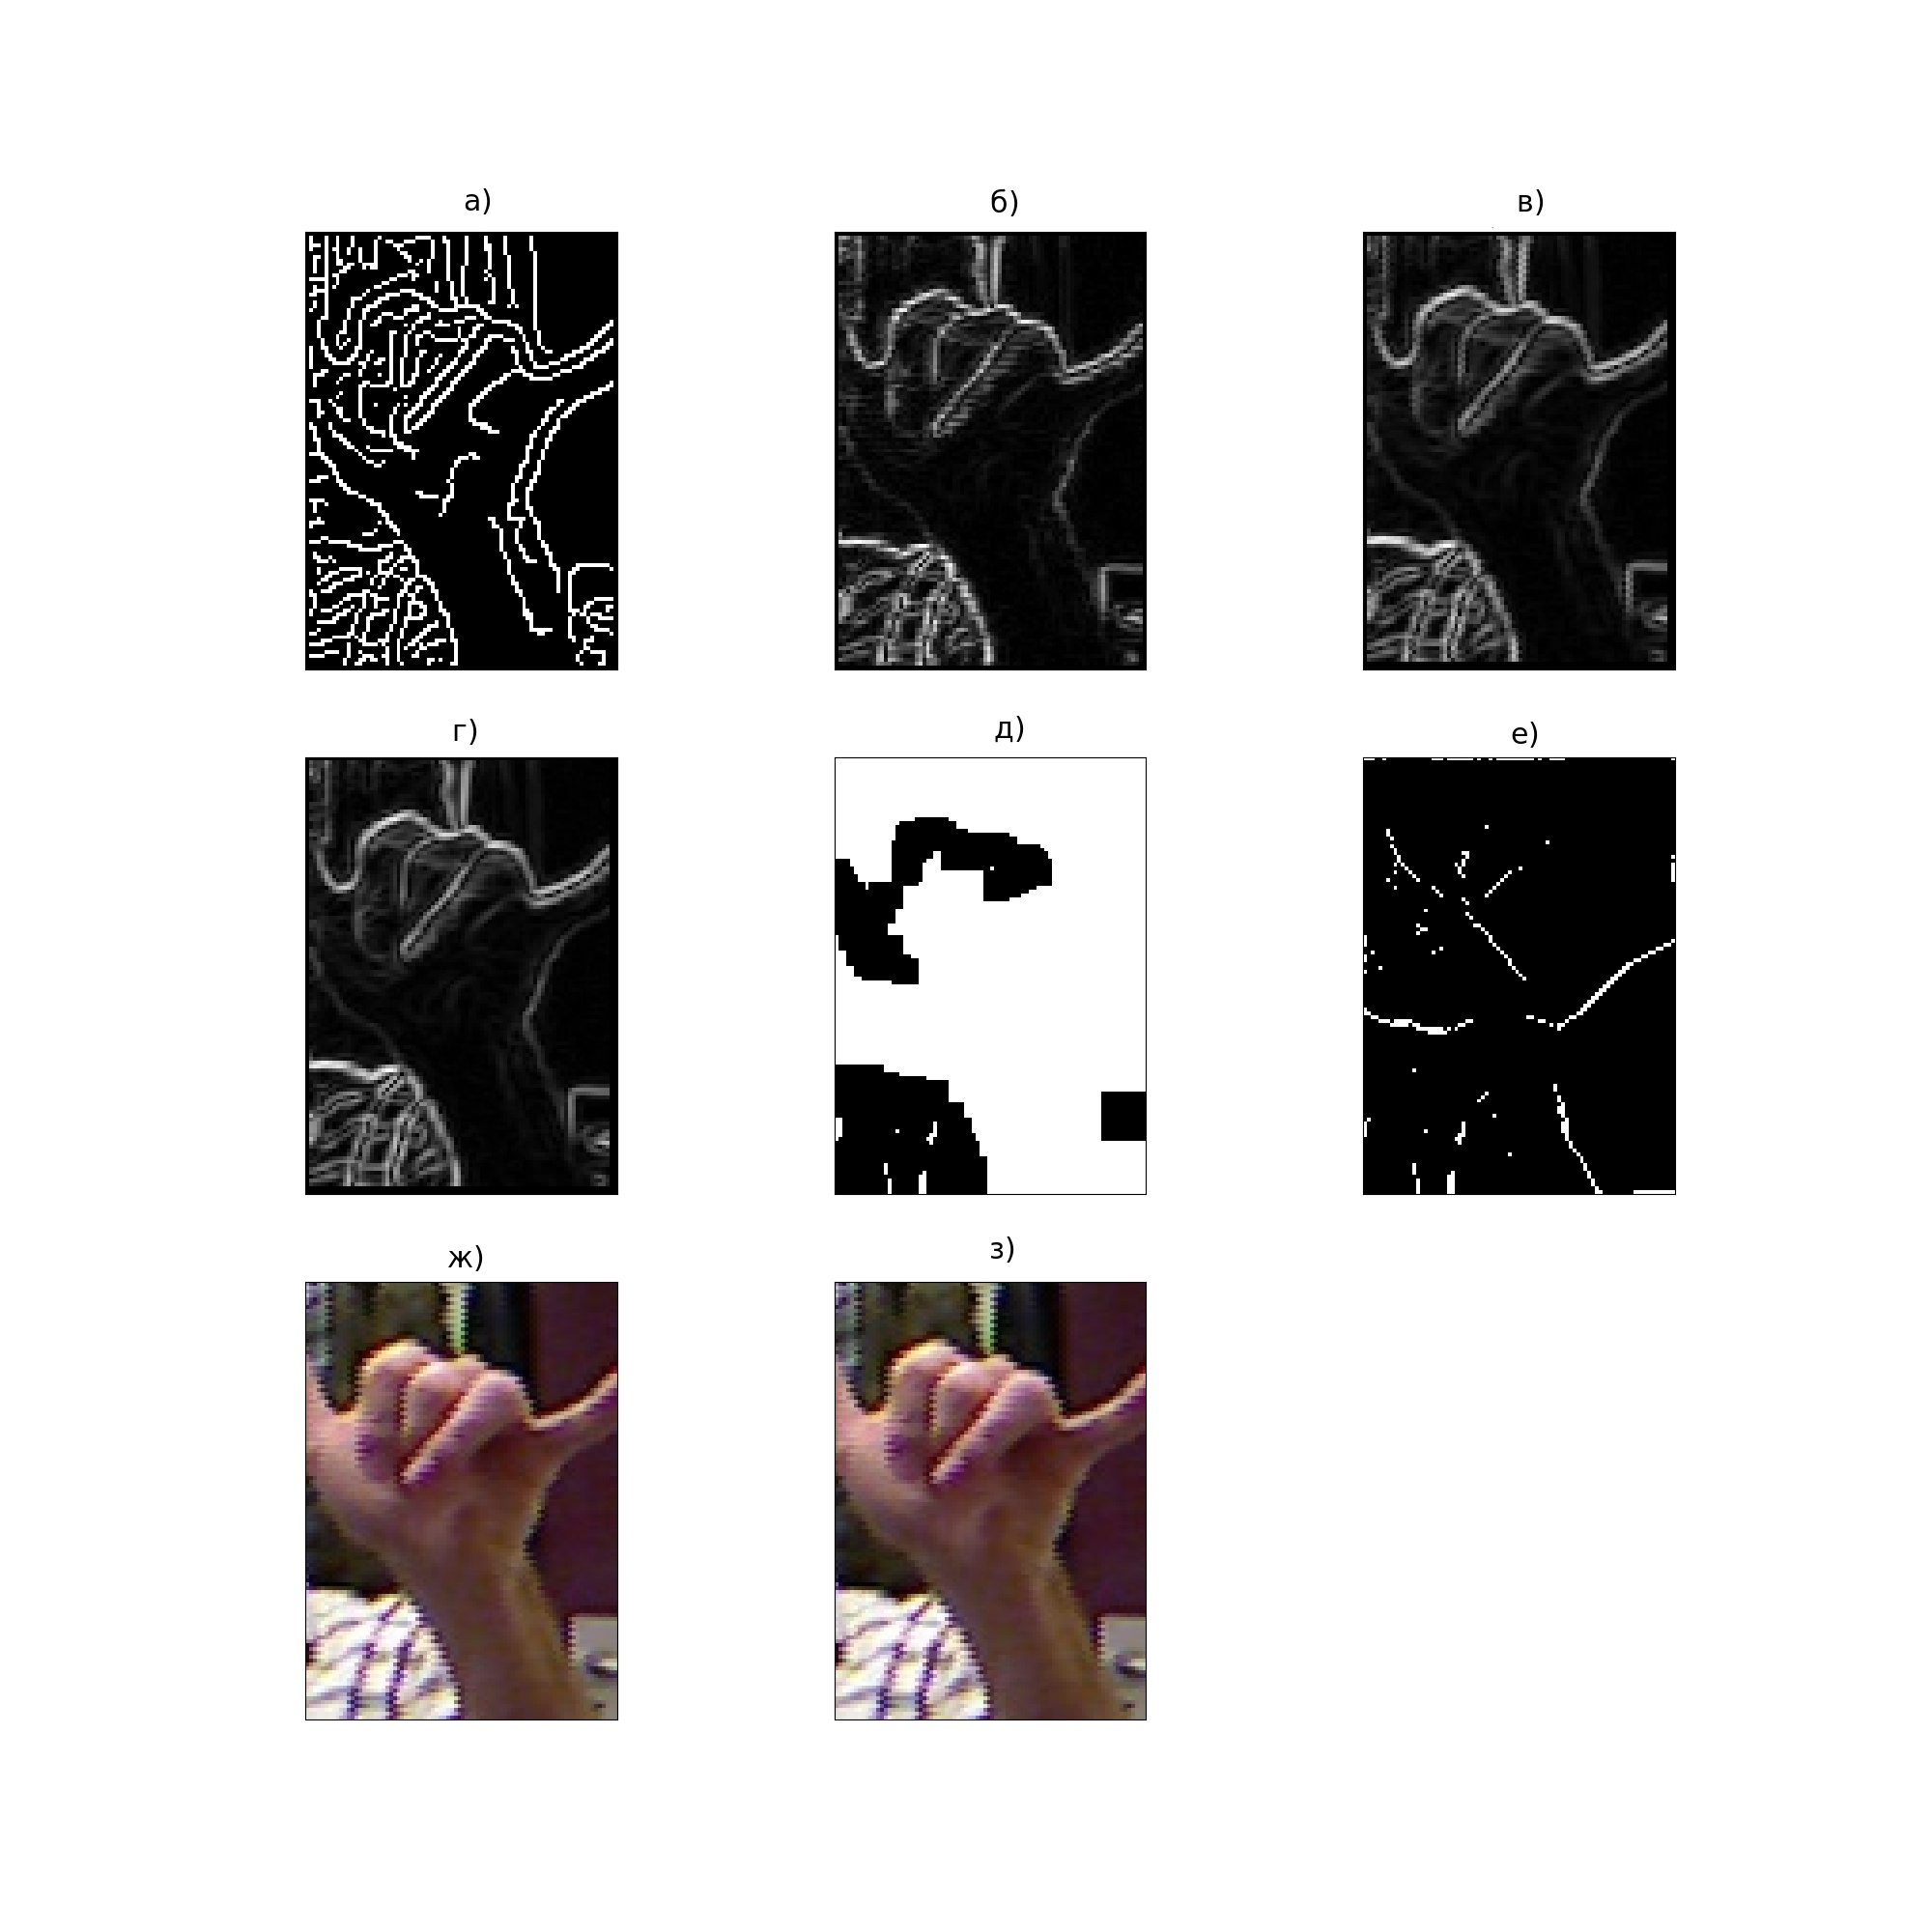
\includegraphics[width=\textwidth]{inc/img/compare1}
	\caption{Результат работы алгоритмов на наборе данных ASL Fingerspelling Images: а) оператор Кэнни; б) оператор Робертса; в) оператор Прюитт; г) оператор Собеля; д) выделение силуэта; е) морфологическое построение скелета; ж) построение скелета по ключевым точкам; з) оригинальное изображение}
	\label{an:compare}
\end{figure}

Морфологическое построение скелета показало время работы, сопоставимое с результатами оператора Кэнни (см. табл. \ref{tab:colombian-alphaber}, \ref{tab:asl2-alphaber}, \ref{tab:datamix-alphaber}). Итоговые результаты обработки изображения данным алгоритмом показали неудовлетворительное качество. Как говорилось выше, в результате получаются побочные ветви, а также скелет получается неполносвязным. В силу данных недостатков практически нецелесообразно использование данного алгоритма в построении метода классификации жестовых символов в силу зашумленности итоговых данных.

Алгоритм построения скелета по ключевым точкам не справился со своей задачей на большинстве изображениях, как видно на рис. 8. Однако, как показано на рис. \ref{an:compare2}, в случае успешного определения ключевых точек алгоритм безупречно производит построение скелетной модели жеста. Также для любого типа данных он работает за одно и то же время. В одних случаях это является преимуществом (табл. \ref{tab:colombian-alphaber}), в других — недостатком (табл. \ref{tab:asl2-alphaber}).

\begin{figure}[!h]
	\centering
	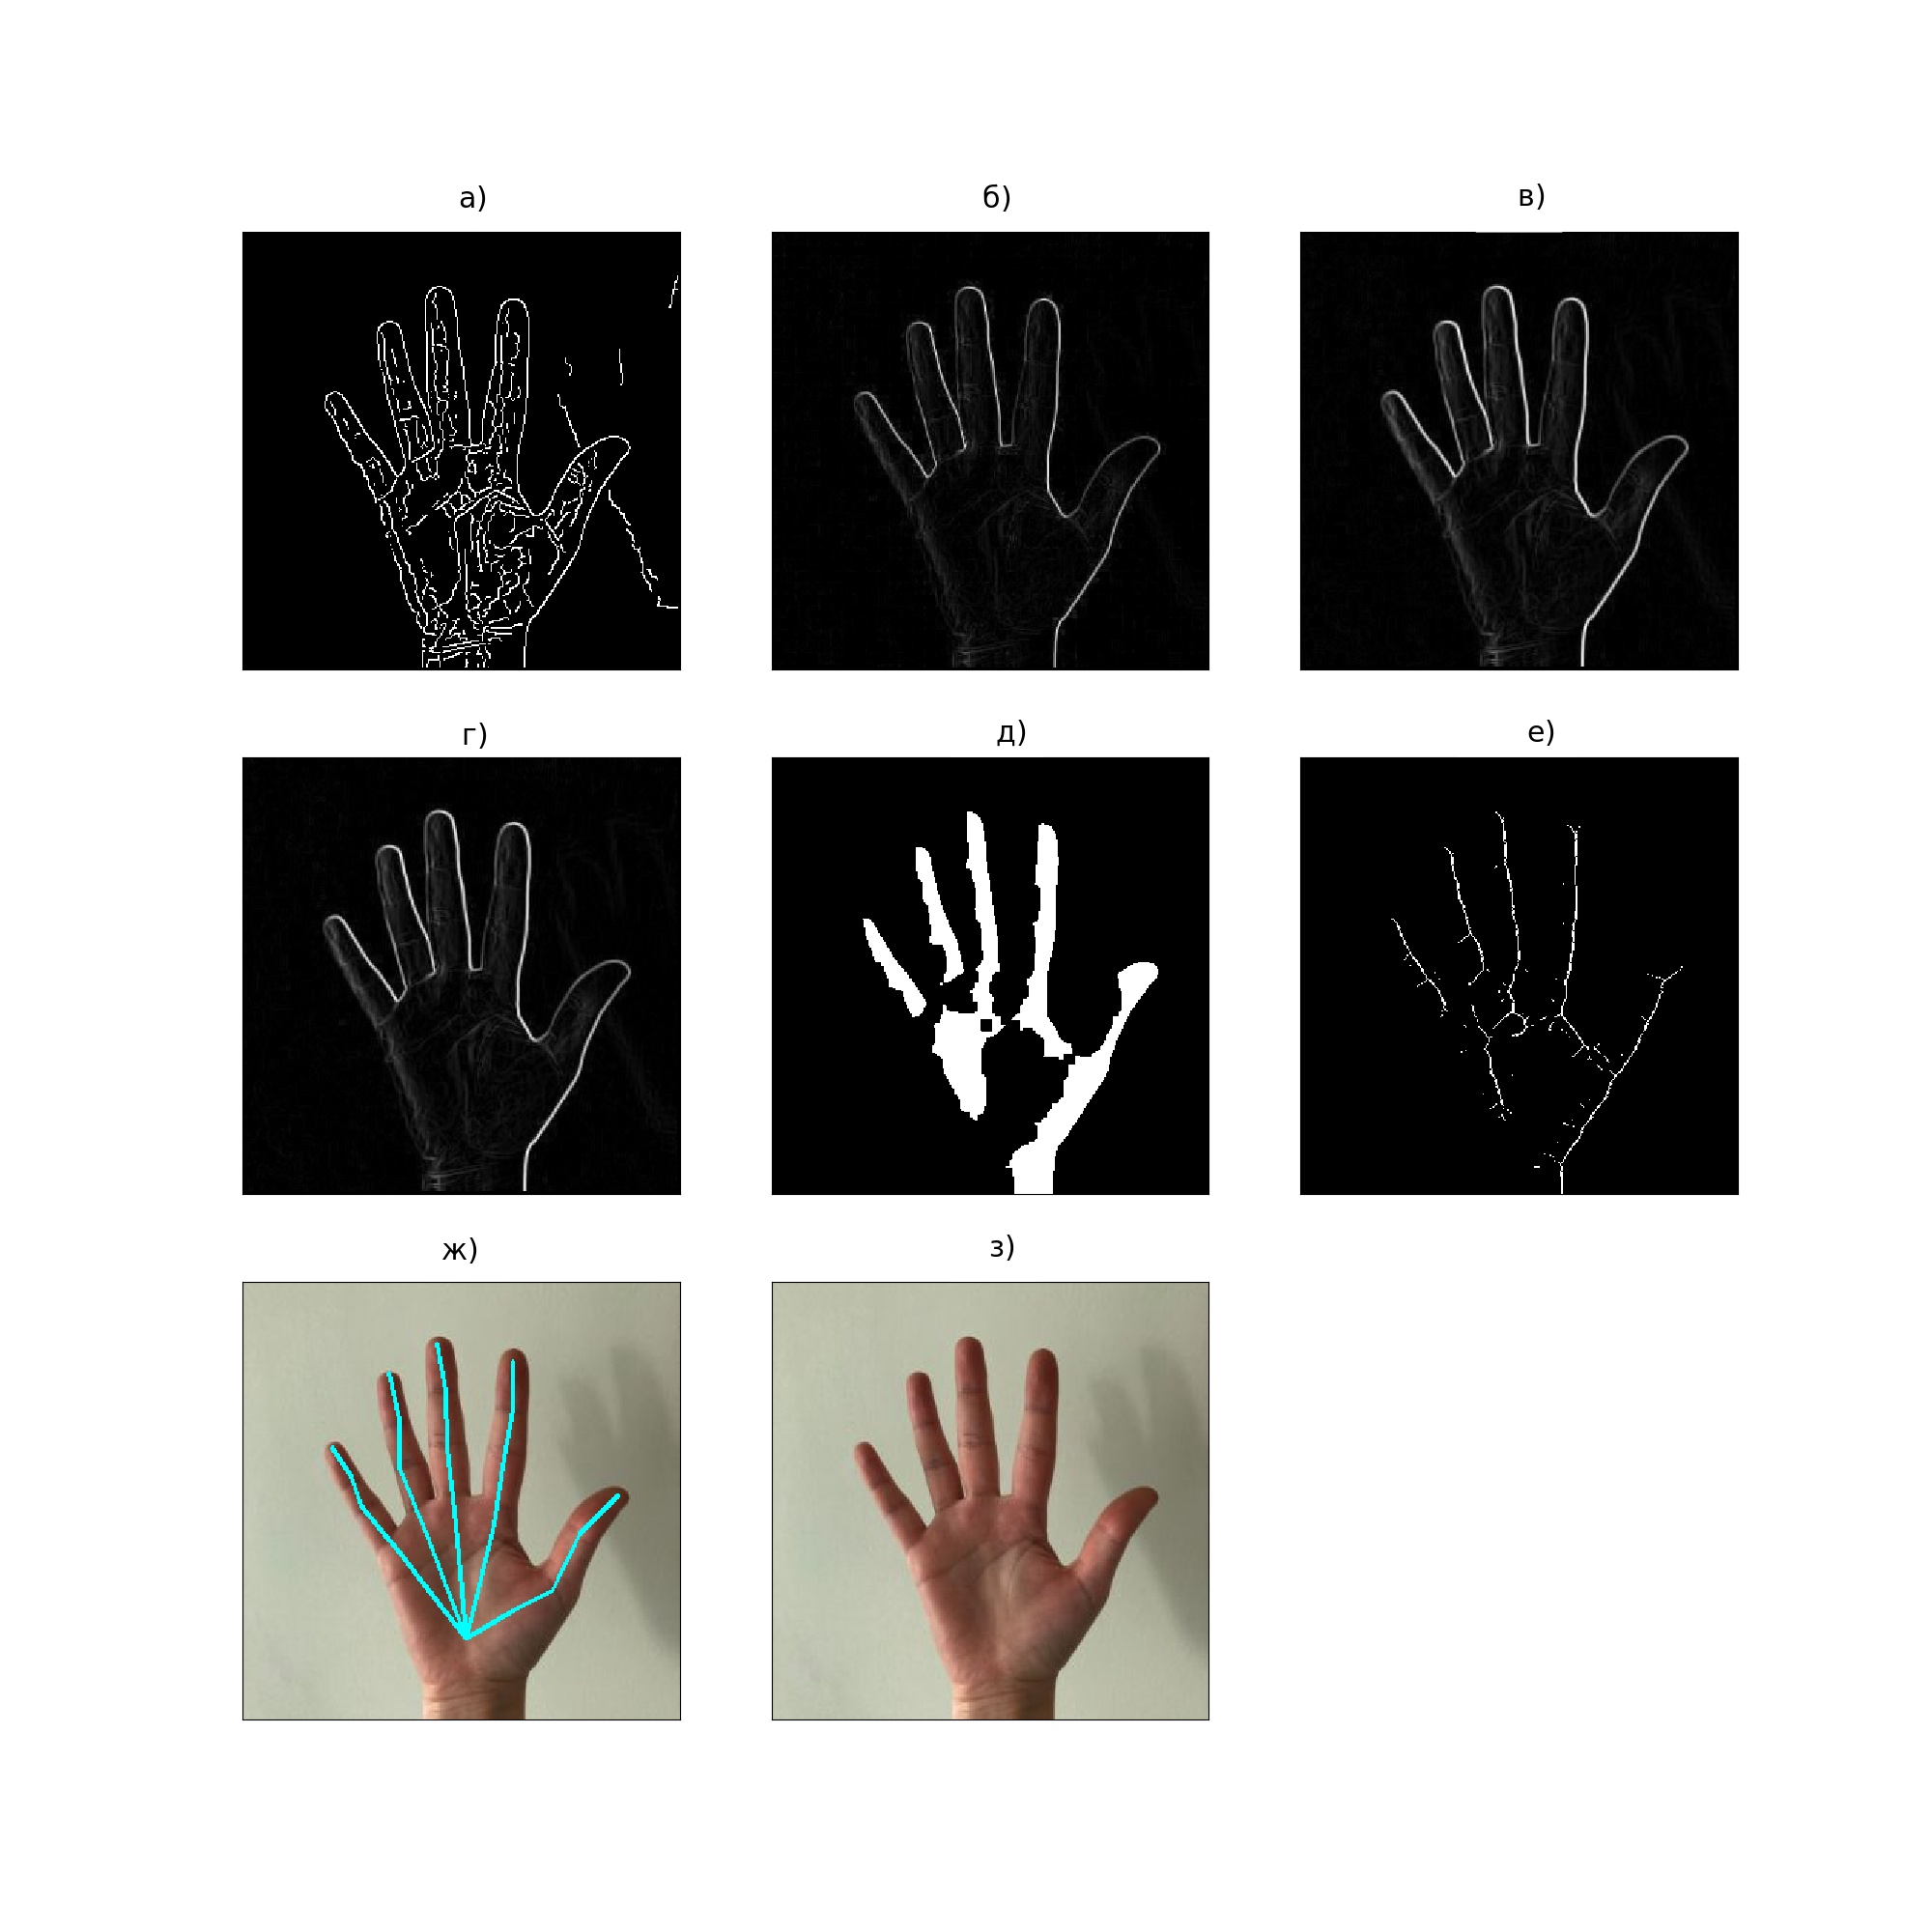
\includegraphics[width=\textwidth]{inc/img/compare2}
	\caption{Результат работы алгоритмов на наборе данных <<sign language between 0 9>>: а) оператор Кэнни; б) оператор Робертса; в) оператор Прюитт; г) оператор Собеля; д) выделение силуэта; е) морфологическое построение скелета; ж) построение скелета по ключевым точкам; з) оригинальное изображение}
	\label{an:compare2}
\end{figure}

\subsection{Вывод}

В результате проведенного сравнительного анализа были определены два метода. 

Выделение силуэта. Данный метод показал наименьшее время работы. Кроме того, бинарное изображение руки содержит в себе необходимые признаки жеста для его обработки классификатором.

Построение скелета по ключевым точкам. Скелетная модель является наилучшим типом входных данных для классификатора, т. к. не несет в себе никаких лишних данных\cite{Gil}.

Первый метод показал наилучшие результаты по скорости работы алгоритма,
кроме тестов на широкоформатных изображениях. В неудачных случаях (рис. \ref{an:compare}) второй метод не смог построить скелетную модель из-за неопределенных ключевых точек жеста.

\section{Методы классификации}

На данный момент известны следующие методы классификации жестовых символов:

\begin{itemize}
	\item скрытая марковская модель\cite{Zhang,Kasprzak};
	\item самоорганизующаяся карта Кохонена\cite{Tewari2012AVR,Karn};
	\item сверточные нейронные сети\cite{Potkin,10.1007/978-3-319-16178-5_40}.
\end{itemize}

\subsection{Скрытая марковская модель}

Одним из методов классификации, широкораспространенный в области распознавания жестов, является скрытая марковская модель (СММ). На ее основе построены системы распознавания китайского\cite{Zhang} и польского\cite{Kasprzak} жестовых языков.

Скрытая марковская модель -- модель процесса, считающегося Марковским. Система представляет собой марковскую цепь, которая имеет конечное множество скрытых состояний, т.е. заданный момент времени неизвестно, в каком состоянии $s_i$ находится система. Каждое состояние $s_i$ может с некоторой вероятностью $b_{io_j}$ произвести событие $o_j$, которое можно наблюдать.

СММ $\lambda$ задается как $\lambda = \{S, \Omega, \Pi, A, B\}$, где $S=\{s_1, ..., s_n\}$ -- множество состояний, $\Omega = \{\omega_1, ..., \omega_m\}$ -- множество возможных событий, $\Pi = \{\pi_1, ..., \pi_n\}$ -- множество начальных вероятностей, $A = \{a_{ij}\}$ -- матрица вероятностей перехода из состояния $s_i$ в состояние $s_j$, $B = \{b_{i\omega_k}\}$ -- множество вероятностей наблюдения события $\omega_k$ после перехода системы в состояние $s_i$.

Задачи, решаемые с помощью СММ можно разделить на следующие группы:

\begin{itemize}
	\item кластерный анализ\cite{Helske} -- упорядочивание объектов в сравнительно однородные группы;
	\item регрессионный анализ\cite{Fridman} -- статистический метод исследования влияния одной или нескольких независимых переменных $x_1, ..., x_n$ на зависимую переменную $y$;
	\item задача классификации\cite{Benyacoub} -- разделение множества объектов некоторым образом на классы.
\end{itemize}

Задачу классификации можно трактовать как поиск вероятности попадания в состояние $s_n$ на шаге $t$. Для этого применяется алгоритм прямого-обратного хода. Обучение модели, происходящее с помощью алгоритма Витерби, заключается в подборе последовательности состояний, при которой вероятность заданной последовательности наблюдений является наибольшей. Алгоритм Баума-Велша меняет коэффициенты матрицы вероятности, максимизируя вероятность наблюдения последовательности событий $O$.

\subsection{Самоорганизующаяся карта Кохонена}

Самоорганизующиеся карты Кохонена(СКК) являются одной из разновидностей искусственных нейронных сетей. В области распознавания жестов нейросети данного типа могут применяться как для предобработки входных данных с целью извлечения признаков для классификатора\cite{Gao}, так и для распознавания самих жестов, например индийского\cite{Tewari2012AVR} и американского\cite{Karn} жестовых языков.

Основным отличием СКК от большинства известных нейронных сетей является обучение без учителя. При данном подходе процесс обучения не требует вмешательства со стороны и по этому результат будет зависеть только от структуры входных данных. Функцией СКК является кластеризация, то есть нет необходимости заранее знать классы выходных данных из обучающей выборки.

Архитектура сети состоит из двух слоев: входного и выходного, при этом каждый нейрон входного слоя связан с каждым нейроном выходного. Нейроны выходного слоя упорядочены и имеют структуру сетки. При этом каждый нейрон представляет собой n-мертный вектор вида $w=[w_1, ..., w_n]^T$, где $n$ равен размерности исходного пространства.

Процесс обучения разделяют на четыре основных этапа:

\begin{enumerate}
	\item Инициализация. Первоначальные веса узлов задаются случайными числами.
	\item Конкуренция. Нейроны вычисляют значения своей функции активации для каждого входного паттерна. Нейрон с наименьшим значением объявляется победителем.
	\item Объединение. Активный нейрон определяет пространственное расположение топологической окрестности нейронов, которые будут участвовать в процессе обучения. Размер окрестности определяется радиусом обучения.
	\item Подстройка весов. Выбранные нейроны уменьшают значения своих функций активации путем регулировки соответствующих весов узлов.
\end{enumerate}

Модификация весовых коэффициентов происходит по формуле \ref{eq:som-weights}.

\begin{eqnarray}\label{eq:som-weights}
w_i(t+1) = w_i(t) + h(t)*[x(t)-w(t)],
\end{eqnarray}

где
\begin{itemize}
	\item $t$ -- номер эпохи;
	\item $x(t)$ -- некоторый вектор из обучающей выборки;
	\item $h(t)$ -- функция соседства нейронов.
\end{itemize}

\subsection{Сверточные нейронные сети}

Создание сверточных нейронных сетей(СНС) было вдохновлено зрительной корой головного мозга человека\cite{Hubel}. Основное использование -- обработка изображений. Отличительной особенностью данной сети, подарившей ей название, является первый скрытый слой, работа которого похожа на процесс свертки двумерного изображения. В связи с этим, для большей наглядности входной слой вместо одномерного слоя нейронов можно рассматривать как двумерную матрицу, как в случае с файлом изображения. Для изображений значения этой двумерной матрицы представляют интенсивности пикселей. 

Рассмотрим особенности данной сети: сверточный и субдискретизирующий слои.

\section*{Слой свертки}

В отличии от обычной нейронной сети, в которой каждый нейрон входного слоя связан с каждым нейроном первого скрытого слоя, в СНС каждый нейрон в скрытом слое, называемом сверточным, связан только с нейронами, находящимися в определенной небольшой области (рис. \ref{anal:CNN-first}), которая определяется ядром свертки. Для формирования скрытого слоя ядро перемещается построчно по всей входной области, и может происходить с различным шагом, например на рисунке \ref{anal:CNN-first} шаг смещения равен 1.

\begin{figure}
	\centering
	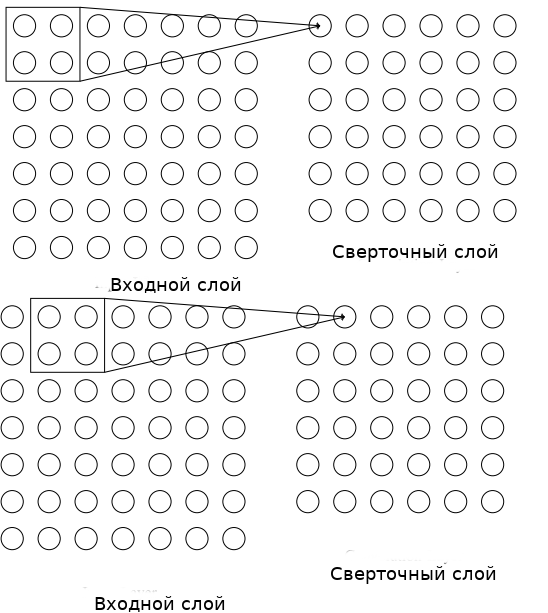
\includegraphics[width=0.6\textwidth]{inc/img/cnn-first.png}
	\caption{Связывание входного слоя с первым скрытым слоем}
	\label{anal:CNN-first}
\end{figure}

Размерность сверточного слоя определяется формулой \ref{eq:cnn-size}.

\begin{eqnarray}\label{eq:cnn-size}
(((W - X) / s) + 1) \times ((H - Y) / s) + 1), 
\end{eqnarray}

где

\begin{itemize}
	\item $W \times H$ -- размерность входного слоя;
	\item $X \times Y$ -- размерность ядра свертки;
	\item $s$ -- шаг смещения.
\end{itemize}

Результат нейрона $j,k$ сверточного слоя описывается формулой \ref{eq:cnn-result}.

\begin{equation}\label{eq:cnn-result}
a_{j,k} = \sigma \Bigg(b + \sum_{l=0}^{A-1} \sum_{m=0}^{B-1} w_{i,m}x_{j+l,k+m}\Bigg)
\end{equation}

Другими словами, сверточный слой выполняет функцию поиска первичных признаков входных данных, например границ изображения.

\section*{Слой субдискретизации}

Слой субдискретизации (англ. Pooling) выполняет задачу уменьшения размерности данных через нелинейное уплотнение. Исходная область разбивается на области, к которым, независимо друг от друга, происходит уплотнение области до одного значения. Пример работы данного слоя предоставлен на рисунке \ref{anal:CNN-pooling}.

\begin{figure}
	\centering
	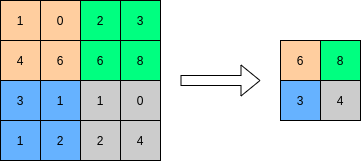
\includegraphics[width=0.6\textwidth]{inc/img/pooling}
	\caption{Cубдискретизация с функцией максимума и фильтром 2$\times$ 2 с шагом 2}
	\label{anal:CNN-pooling}
\end{figure}

Размер области задается фильтром, который обычно равен $2 \times 2$. В качестве функции фильтра обычно используют функцию максимума. Но так же применимы и другие, например функции среднего значения и L2-нормирования. 

Другими словами работу слоя субдискретизации можно описать следующим образом: если при работе сверточного слоя уже были выявлены некоторые признаки, то в дальнейшем настолько подробные данные уже не нужны, то есть можно их сократить до менее подробных.

\section*{Общая архитектура СНС}

В задачах распознавания жестовых символов СНС уже применялась для работы с русским\cite{Potkin} и итальянским\cite{10.1007/978-3-319-16178-5_40} жестовыми языками. Не смотря на разницу в архитектурных особенностях методов, общий подход к построению сети можно разделить на следующие слои:

\begin{enumerate}
	\item Сверточный слой.
	\item Слой субдискретизации.
	\item Полносвязный слой.
\end{enumerate}

\subsection{Сравнительный анализ выделенных методов классификации}

В результате анализа предметной области были рассмотрены три метода классификации жестовых символов. Каждый класс обладает рядом функциональных преимуществ, которые выделяют его на фоне других подходов. В то же время имеется и ряд недостатков, который ограничивает область применимости данно­го класса методов.

Сравнение преимуществ и недостатков рассмотренных решений представлено в таблице \ref{anal:longtable-classificators}.

\begin{center}
	\begin{longtable}{|p{0.30\textwidth}|p{0.32\textwidth}|p{0.32\textwidth}|}
		\caption{Сравнительный анализ методов классификации}
		\label{anal:longtable-classificators}
		\\ \hline
		Название метода & Преимущества & Недостатки \\
		\hline \endfirsthead
		\subcaption{Продолжение таблицы~\ref{anal:longtable-classificators}}
		\\ \hline \endhead
		\hline \subcaption{Продолжение на след. стр.}
		\endfoot
		\hline \endlastfoot
		СММ & Простая математическая структура & Каждая модель обучается только на экземплярах своего класса \\
		& Возможность использования исходных данных без предобработки & Большое число неструктурированных параметров \\
		&& Максимизация отклика модели на свои классы без минимизации на другие \\
		\hline
		Самоорганизующаяся карта Кохонена & Обучение без учителя & Окончательный результат зависит от начальных установок \\
		& Устойчивость к зашумленным данным &\\
		& Скорость обучения &\\
		\hline
		СНС & Частичная инвариантность к масштабу & Склонность к переобучению \\
		& Частичная инвариантность к повороту и сдвигу & Необходимость в большой обучающей выборке \\
		& Созданы специально для обработки изображений &  \\
	\end{longtable}
\end{center}

Сравнительный анализ качества классификации на американском жестовом языке выделенных методов представлено в таблице \ref{anal:longtable-accuracy}.

\begin{center}
	\begin{longtable}{|p{0.60\textwidth}|c|}
		\caption{Точность работы методов классификации}
		\label{anal:longtable-accuracy}
		\\ \hline
		Название метода & Точность \\
		\hline \endfirsthead
		\subcaption{Продолжение таблицы~\ref{anal:longtable-accuracy}}
		\\ \hline \endhead
		\hline \subcaption{Продолжение на след. стр.}
		\endfoot
		\hline \endlastfoot
		СММ\cite{Starner} & 90,7 -- 93,5\%  \\
		\hline
		Самоорганизующаяся карта Кохонена\cite{Karn}& 92\% \\
		\hline
		СНС\cite{Garcia} & 97,82\% \\
	\end{longtable}
\end{center}

Как видно из таблицы, использование СНС дает наилучший результат классификации в задачах распознавания жестовых символов. Данный тип нейронной сети изначально рассчитан на обработку изображений. 

\subsection{Капсульные нейронные сети}

Капсульные нейронные сети (англ Capsule Neural Network) -- предназначенная для распознавания изображений архитектура нейронных сетей. КНС были задуманы Джеффри Хинтоном в 1979 году, первые работы по ней опубликованы в 2017 году\cite{sabour2017dynamic}. Идея данной сети является следствием критики сверточных нейронных сетей. Полученная в ходе свертки информация о входных данных частично теряется на этапе субдискретизации. Например в задачи распознавания лиц данная сеть учитывает наличие на изображении глаз, ушей, носа и губ, но игнорирует их взаимное расположение. Следствием этого может быть ложное распознавание деформированного лица, пример которого представлен на рисунке \ref{anal:CNN-bad}.

\begin{figure}
	\centering
	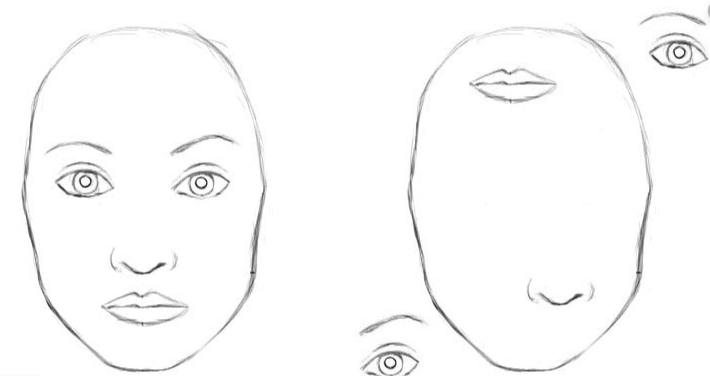
\includegraphics[width=0.8\textwidth]{inc/img/face_deformed}
	\caption{Деформированное изображение лица}
	\label{anal:CNN-bad}
\end{figure}

Особенностью КНС являются капсулы -- группа нейронов, инкапсулирующая информацию о состоянии функции, которую обнаруживают в векторной форме. 

В отличии от обычных нейронов, работающих со скалярными величинами, капсулы работают с векторами. Вычисление выходного значения капсулы происходит в соответствии с формулой \ref{eq:caps-sum}, представляющее собой скалярное произведение векторов.

\begin{eqnarray}\label{eq:caps-sum}
s_j = \sum_{i}c_{ij}\hat{u}_{i|j} \quad	\hat{u}_{i|j} = W_{ij}u_i,
\end{eqnarray}

где

\begin{itemize}
	\item $u_i$ -- вектор входных значений;
	\item $W_{ij}$ -- матрица аффинного преобразования;
	\item $c_{ij}$ -- коэффициент маршрутизации;
	\item $s_j$ -- выходное значение.
\end{itemize}

Заменой функции активизации, применяемой в нейронах для задания нелинейности данным, в капсулах является нормализация нормализация выходного вектора по формуле \ref{eq:caps-norm}.


\begin{eqnarray}\label{eq:caps-norm}
v_j = \frac{{||s_j||}^2}{1 + {||s_j||}^2} \frac{s_j}{||s_j||}
\end{eqnarray}

Итоговые различия между капсулами и обычными нейронами представлена в таблице \ref{tab:caps2trad}.

\begin{table}[!h]
	\caption{\label{tab:caps2trad}Различия между капсулами и нейронами}
	\begin{center}
		\begin{tabular}{|c|c|c|}
			\hline
			Параметр & Капсула & Нейрон \\
			\hline
			Формат входных данных & вектор $(u_i)$ & скаляр $(x_i)$ \\
			\hline
			Преобразование входных данных & $\hat{u}_{i|j} = W_{ij}u_i$ & -- \\
			\hline
			Сумматор & $s_j = \sum_{i}c_{ij}\hat{u}_{i|j}$ & $a_j = \sum_{i}w_ix_i + b$ \\
			\hline
			Передаточная функция & $v_j=\frac{{||s_j||}^2}{1 + {||s_j||}^2}\frac{s_j}{||s_j||}$ & $h_j=f(a_j)$ \\
			\hline
			Формат выходных значений & вектор $(v_j)$ & скаляр $(h_j)$ \\
			\hline
		\end{tabular}
	\end{center}
\end{table}

Капсулы являются расширением нейронов до векторной формы, что позволяет хранить, обрабатывать и передавать больше информации. Например в задачах распознавания лиц капсула может хранить не только признаки присутствия глаза на изображении, но и дополнительную информацию о его положении относительно других частей.

Благодаря этим особенностям данная архитектура инвариантна к поворотам и смещениям изображения, обучение происходит быстрее и требует меньший объем выборки. Применение данной архитектуры позволяет сократить ошибку классификации при поворотах на 43\%, в сравнении с СНС\cite{em}. Эти утверждения были экспериментально доказаны на датасете рукописных цифр MNIST\cite{sabour2017dynamic}.

Автор предлагает использование КНС в качестве классификатора при построении метода классификации жестовых символов.

\section{Вывод}

Были представлены этапы работы известных методов распознавания жестовых символов. Рассмотрены возможные способы получения информации, их преимущества и недостатки. 

Проведен сравнительный анализ методов предобработки изображений. Показано преимущество выделения силуэта кисти руки в сравнении с остальными методами с точки зрения скорости и качества выделения признаков с изображения.

Сравнительный анализ методов классификации показал, что СНС имеет наилучшее качество распознавания среди рассмотренных классификаторов. Принято решение использование данного решения в качестве базового при построении метода распознавания жестовых символов. Не смотря на высокую точность классификации, СНС имеют проблемы с инвариантностью к пространственным изменениям изображения, а так же требуют большого объема обучающей выборки. В качестве альтернативы предложено использование КНС, архитектура которых направлена на устранение описанных недостатков сверточных сетей.
\chapter{Конструкторский раздел}
\label{cha:design}

\section{Архитектура программного продукта}

Разрабатываемый метод состоит из 2 частей:

\begin{enumerate}
	\item модуль предобработки входных данных;
	\item модуль классификации жестового символа.
\end{enumerate}

В качестве входных данных используются RGB изображения. Данный формат данных может быть получен с любого фото- и видео-устройства.

\section{Предобработка изображений}

В рассмотренном ранее методе выделения силуэта кисти руки предлагалась фильтрация пикселей изображения в цветовом пространстве YCbCr. Как показывает практика, данное решение имеет недостаток в виде артефактов выделения. Данная проблема возникает из-за наличия в фоновой части изображения пикселей, цвет которых близок к цвету кожи в данном цветовом пространстве.

Избежать подобные дефекты можно через дополнительную фильтрацию в цветовом пространстве HSV\cite{Kolkur}. В итоговом методе пиксели исходного изображения проверяются одновременно и в обоих цветовых пространствах. 

Для преобразования изображения из RGB в YCbCr используется формула \ref{eq:ycbcr}.

\begin{eqnarray}\label{eq:ycbcr}
\begin{bmatrix}
Y\\Cb\\Cr
\end{bmatrix}
=
\begin{bmatrix}
16\\128\\128
\end{bmatrix}
+
\begin{bmatrix}
65,81 & 128,551 & 24,966 \\
-37,797 & -74,203 & 112\\
112 & -93,786 & -18,214
\end{bmatrix}
\begin{bmatrix}
R\\G\\B
\end{bmatrix}
\end{eqnarray}

В HSV координатами цвета являются:

\begin{itemize}
	\item H -- цветовой тон, интервал значений $0 - 360^\circ$;
	\item S -- насыщенность, $0 - 1$;
	\item V -- яркость, $0 - 1$;
\end{itemize}

Для получение значения координат пикселя в пространстве HSV, нормализуем его координаты в RGB по максимальному значению.
\begin{equation}
R'=R/255 \quad G'=G/255 \quad B'=B/255
\end{equation}

Зададим так же 
\begin{equation}
C_{max} = max(R', G', B')
\end{equation}

\begin{equation}
C_{min} = min(R', G', B')
\end{equation}

\begin{equation}
\Delta = C_{max} - C_{min}.
\end{equation}

Тогда координаты пикселя в пространстве HSV вычисляются следующим образом:

\begin{eqnarray}
\begin{matrix}
H & =
& \left\{
\begin{matrix}
0^\circ &, \Delta = 0 \\
60^\circ \times ( \frac{G' - B'}{\Delta} \mod 6 )& , C_{max} = R' \\
60^\circ \times ( \frac{B' - R'}{\Delta} + 2)& , C_{max} = G' \\
60^\circ \times ( \frac{R' - G'}{\Delta} + 4)& , C_{max} = B' \\
\end{matrix} \right.
\end{matrix}
\end{eqnarray}

\begin{eqnarray}
\begin{matrix}
S & =
& \left\{
\begin{matrix}
0 &, C_{max} = 0 \\
\frac{\Delta}{C_{max}} &,C_{max} \ne 0
\end{matrix} \right.
\end{matrix}
\end{eqnarray}

\begin{eqnarray}
V = C_{max}
\end{eqnarray}

Алгоритм \ref{des:image_mask} описывает процесс получения силуэта кисти руки.

\begin{algorithm}[H]
	\label{des:image_mask}
	\SetAlgoLined
	\KwIn{Изображение $x$}
	\KwOut{Однотонное черно-белое изображение $y$}	
	
	Получить изображение в YCbCr
	
	$x_{ycbcr} \leftarrow YCbCr(x)$
	
	Получить изображение в HSV
	
	$x_{hsv} \leftarrow HSV(x)$
	
	\ForEach{пикселя p изображения x с координатами i, j}{
		$Y =$ значение $Y$ пикселя $x_{ycbcr}$
		
		$Cb =$ значение  $Cb$ пикселя $x_{ycbcr}$
		
		$Cr =$ значение  $Cr$ пикселя $x_{ycbcr}$
		
		$H =$ значение $H$ пикселя $x_{hsv}$
		
		$S =$ значение  $S$ пикселя $x_{hsv}$
		
		$V =$ значение  $V$ пикселя $x_{hsv}$
		
		\If{
			$Y > 80$ и
			$ 135 \le Cr \le 180 $ и
			$ 85 \le Cb \le 135 $ и
			$ H \le 50^\circ $ и 
			$ 0,23 \le S \le 0,68 $
		}{
			$y[i][j] = 255$
		} \Else{
			$y[i][j] = 0$
		}
	}
	
	\caption{Алгоритм выделения силуэта кисти руки}
\end{algorithm}

\section{Классификация жестовых символов}

Ранее было показано преимущество использование СНС в качестве классификатора в известных методах распознавания жестовых символов, выделены недостатки данного метода. Предложено использование КНС в качестве альтернативы с целью уменьшения обучающей выборки, ускорения процесса обучения и добавления методу инвариантности к аффинным преобразованиям изображения.

\subsection{Алгоритм передачи данных между капсульными слоями}

Передача информации между капсульными слоями происходит с помощью динамической маршрутизации. Целью данного алгоритма является передача выхода низкоуровневых капсул только тем капсулам, которые способны на основании полученных данных получить наилучший результат в контексте решаемой данной архитектурой задачи. 

Все входные вектора капсулы после аффинного преобразования умножаются на коэффициенты маршрутизации, сумма которых равна единице. Значения данных коэффициентов задаются функцией softmax (формула \ref{eq:softmax}).

\begin{equation}\label{eq:softmax}
c_{ij} = \frac{e^{b_{ij}}}{\sum_{k}e^{b_{ik}}}
\end{equation}

Значение неизвестных $b_{ij}$ вычисляются дискриминативно одновременно с остальными весовыми коэффициентами. Данный процесс зависит исключительно от взаимного расположения и типа капсул и не зависит от входных данных. Начальные коэффициенты связи затем итеративно уточняются на основании согласованности текущих выходов $v_j$ низкоуровневых капсул $j$ и предсказанием $\hat{u}_{i|j}$ высокоуровневой капсулы $i$.

Согласованность между капсулами определяется скалярным произведением $a_{ij} = v_j \hat{u}_{j|i}$. Оно рассматривается как логарифмическая вероятность и добавляется к исходному значению $b_{ij}$  перед вычислением новых значений для всех коэффициентов связи, связывающих капсулу $i$ с капсулами более низкого уровня.

Алгоритм \ref{alg:routing} описывает итерационный процесс вычисления коэффициентов связи.

\begin{algorithm}[H]
	\label{alg:routing}
	\SetAlgoLined
	\KwIn{Вектор $\hat{u}_{j|i}$, количество итераций $r$, капсульный слой $l$}
	\ForEach{индекса $i$ капсулы слоя $l$ и индекса $j$ капсулы слоя $l+1$}{$b_{ij} \leftarrow 0$}
	\For{ r итераций}{
		\ForEach{индекса $i$ капсулы слоя $l$}{$c_{ij} \leftarrow softmax(b_{ij})$}
		\ForEach{индекса $j$ капсулы слоя $l+1$}{$s_j = \sum_{i}c_{ij}\hat{u}_{j|i}$}
		\ForEach{индекса $j$ капсулы слоя $l+1$}{$v_j=\frac{{||s_j||}^2}{1 + {||s_j||}^2}\frac{s_j}{||s_j||}$}
		\ForEach{индекса $i$ капсулы слоя $l$ и индекса $j$ капсулы слоя $l+1$}{$b_{ij} \leftarrow b_{ij} + v_j \hat{u}_{j|i}$}
	}
	\caption{Алгоритм динамической маршрутизации}
\end{algorithm}


\subsection{Архитектура сети}

Архитектура сети состоит из 4 слоев:

\begin{enumerate}
	\item Входной слой. На вход сети подается черно-белое одноканальное изображение, где каждое значение пикселя означает интенсивность белого цвета.
	\item Сверточный слой. Имеет 256 фильтров размерностью $9 \times 9$ со смещением 1.	В качестве активационной функции используется ReLU (формула \ref{anal:relu}).
	\begin{equation}
	x_{k} = \max(u_{k}, 0), k = 1, ..., K
	\label{anal:relu}
	\end{equation}
	где 
	\begin{itemize}
		\item $x_k$ -- выходное значение нейрона $k$-го слоя;
		\item $u_k$ -- результат работы сумматора нейрона $k$-го слоя.
	\end{itemize}
	\item Первый капсульный слой. Состоит из 32 капсул, каждая из которых представляет собой набор из 8 сверточных слоев с дает на выходе $N \times N$ векторов длины 8, где $N$ - число строк или столбцов матрицы, полученной в результате свертки. Ядро свертки имеет размерность $9 \times 9$ со смещением 2. Условно, данную капсулу можно представить в виде группы подкапсул, объединенных одним набором весовых коэффициентов.
	\item Выходной капсульный слой. Состоит из $J$ капсул, где $J$ -- количество классов. Выходной вектор имеет длину 8. Каждая капсула принимает на вход все выходы с предыдущего слоя с применением алгоритма динамической маршрутизации. Для большей наглядности данный слой можно интерпретировать как полносвязный в СНС. Длина выходного вектора капсулы на данном слое соответствует вероятности принадлежности входных данных к классу, представленному конкретной капсулой, то есть итоговый класс изображения определяется по капсуле с выходным вектором наибольшей длины.
\end{enumerate}

Схема нейронной сети представлена на рисунке \ref{design:CapsNet}.

\begin{figure}
	\centering
	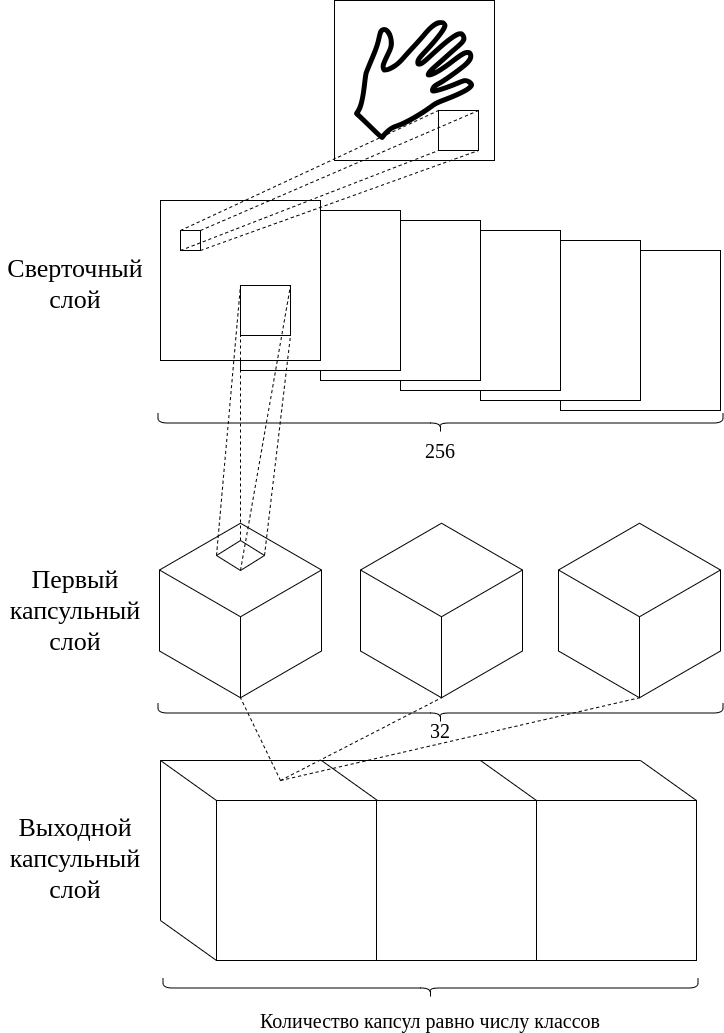
\includegraphics[width=\textwidth]{inc/img/CapsNet}
	\caption{Архитектура капсульной нейронной сети}
	\label{design:CapsNet}
\end{figure}

Ошибка обучения вычисляется для каждой капсулы выходного слоя по следующей формуле:

\begin{equation}
\label{eq:magin-loss}
L_k = T_k \max (0, m^+ - ||v_k||)^2 + \lambda (1 - T_k) \max (0, ||v_k|| - m^-)^2
\end{equation}

где

\begin{itemize}
	\item $L_k$ -- ошибка $k$ - ой капсулы;
	\item $T_k$ равен 1, если $k$-я капсула представляет текущий класс, иначе равен 0;
	\item $m^+, m^-$ -- варьируемые коэффициенты. В данной работе использовались значения 0,9 и 0,1 соответственно;
	\item $\lambda$ -- коэффициент уменьшения исходных весов для отсутствующих классов, исключающий из процесса обучения сокращение длины вектора активности для всех сущностей. В данной работе используется значение 0,5.
\end{itemize}

Итоговая ошибка обучения вычисляется как сумма $L = \sum_{k} L_k$.

\section{Вывод}

В конструкторском разделе описывается построение метода распознавания жестовых символов. Дано подробное описание, построены схемы выбранных алгоритмов. При этом выделены основные этапы работы метода с указанием необходимых исходных данных для его работы и полученных результатов на каждом этапе.
\chapter{Технологический раздел}
\label{cha:impl}

В данном разделе описываются средства, используемые для разработки программного реализации построенного метода, требования для функционирования ПО, описываются результаты тестирования программного продукта.

\section{Выбор средств разработки}

\subsection{Выбор языка программирования}

Для программной реализации описанного метода был выбран язык программирования Python, так как он обладает следующими свойствами:

\begin{itemize}
	\item большая база библиотек для работы с искусственными нейронными сетями, изображениями и математических расчетов;
	\item сочетание функционального, структурного и объектно-ориентированного подходов позволяет кратко описывать необходимые для решения поставленной задачи математические структуры;
	\item кроссплатформенность.
\end{itemize}

Описанные особенности позволяют при помощи Python одинаково удобно реализовывать как научно-исследовательские прототипы, так и коммерческие реализации программного продукта.

\subsection{Выбор среды программирования и отладки}

В качестве среды разработки для языка Python была выбрана кроссплатформенная IDE PyCharm, выбор которой обусловлен следующими предоставляемыми возможностями, упрощающими разработку приложения и способствующими повышению качества исходного кода:

\begin{itemize}
	\item рефакторинг;
	\item навигация по проекту и исходному коду;
	\item встроенный отладчик;
	\item поддержка систем контроля версий;
	\item статический анализ кода.
\end{itemize}

\subsection{Используемые библиотеки}

В процессе реализации были использованы следующие библиотеки:

\begin{itemize}
	\item OpenCV -- библиотека для обработки изображений. Использовалась для считывания, записи и реализации предобработки входных данных.
	\item scikit-learn -- библиотека для машинного обучения. Используется для форматирования входных данных.
	\item NumPy -- библиотека реализаций вычислительных алгоритмов, оптимизированных для работы с многомерными массивами. Используется для упрощения реализации математических операций.
	\item Tensorflow -- библиотека для машинного обучения. Используется для построения и обучения классификатора.
	\item Keras -- библиотека машинного обучения. Используется для построения модели классификатора, работающий на базе Tensorflow.
	\item Tkinter -- графическая библиотека. Используется для создания пользовательского интерфейса на базе средств Tk.
\end{itemize}

\section{Система контроля версий}

В процессе разработки программы использовалась система контроля версий Git, позволяющая вносить в проект атомарные изменения, направленные на решения каких-либо задач. В случае обнаружения ошибок или изменения требований, внесенные изменения можно отменить. Кроме того, с помощью системы контроля версий решается вопрос резервного копирования.

Особенности Git:

\begin{itemize}
	\item данная система контроля версий является децентрализованной, что позволяет иметь несколько независимых резервных копий проекта;
	\item поддерживается хостингом репозиториев GitHub;
	\item поддерживается средой разработки PyCharm;
	\item предоставляет широкие возможности для управления изменениями проекта и просмотра истории изменений.
\end{itemize}

\section{Требования к вычислительной системе}

Для запуска программы необходимо иметь установленный на ЭВМ интерпретатор для Python 3.6 с установленными библиотеками. 

Так как выбранный язык программирования является кроссплатформенным, то требований к использованию операционной системы нет.

Обрабатываемые изображения не требуют большого объема оперативной памяти, но классификатор работает с большим числом параметров, поэтому рекомендуемый размер ОЗУ составляет не менее 256 Мб, желательна архитектура x64 (x86-64).

\section{Формат данных}

В качестве входных данных используются RGB изображения в следующих форматах:

\begin{itemize}
	\item BMP -- разработка компании Microsoft. В данном формате хранятся только однослойные растры. Значения пикселей могут иметь разрядности 1, 2, 4, 8, 16, 24, 32, 48 и 64 бит. При 8 и меньше бит в пикселе хранится индекс цвета в таблице цветов, а при большей -- непосредственное значение в цветовой модели RGB.
	\item JPEG -- формат хранения растровых изображений, способный сжимать изображения как с потерями, так и без потерь качества. 
	\item PNG -- графический формат, отличительной способностью которого является возможность хранения значений альфа-канала, отвечающую за прозрачность пикселя.
\end{itemize}

\section{Проектирование архитектуры программного комплекса}

Разрабатываемый программный комплекс состоит из следующих частей:

\begin{itemize}
	\item модуль получения изображения жеста;
	\item модуль предобработки входных данных;
	\item модуль классификации жеста.
\end{itemize}

Формальная модель системы изображена на рисунке \ref{impl:idef0}.

\begin{figure}[!h]
	\centering
	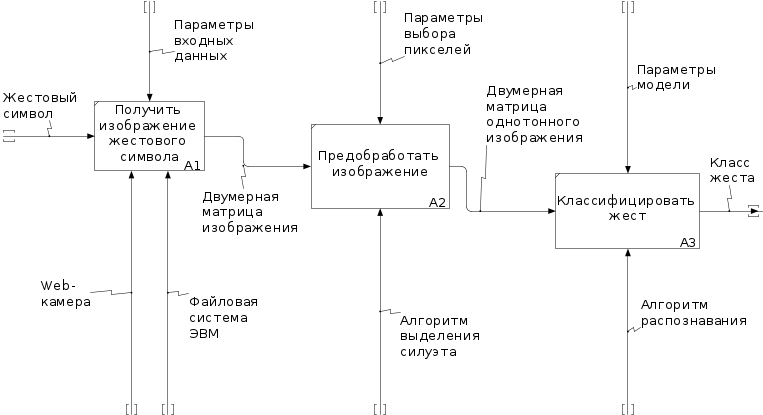
\includegraphics[width=\textwidth]{inc/img/idef0}
	\caption{Формальная модель системы классификации жестовых символов}
	\label{impl:idef0}
\end{figure}

Функционал обучения системы и распознавания жестов разделен на две отдельные подсистемы, объединенных единым хранилищем моделей, из-за разного подхода обработки данных. Итоговая архитектура программного комплекса представлена на рисунке \ref{impl:arch}.

\begin{figure}[!h]
	\centering
	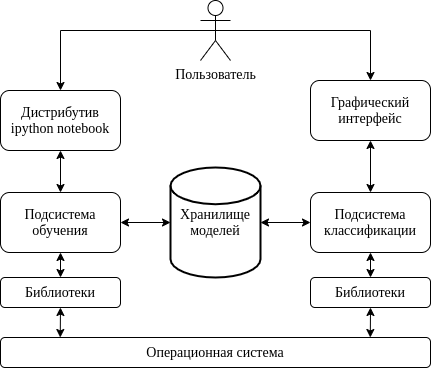
\includegraphics[width=0.55\textwidth]{inc/img/arch}
	\caption{Архитектура программного комплекса}
	\label{impl:arch}
\end{figure}

Основной задачей системы обучения является подготовка моделей классификатора для определенного набора жестовых символов. Для исследования эффективности этапа предобработки входных данных, подсистема обучения способна создавать модели для изображений с предобработкой и без. Функциональные возможности подсистемы обучения представлены на рисунке \ref{impl:train_func}.

\begin{figure}[!h]
	\centering
	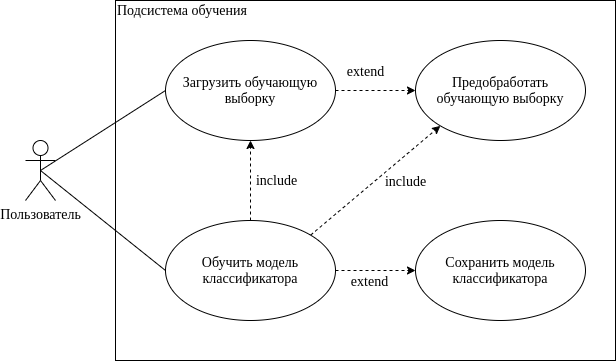
\includegraphics[width=0.6\textwidth]{inc/img/train_func}
	\caption{Функциональные возможности подсистемы обучения}
	\label{impl:train_func}
\end{figure}

Подсистема распознавания жестовых символов выполняет получение изображения с жесткого диска или с Web-камеры, предобработку данных и классификацию жеста. Функциональные возможности подсистемы распознавания жестовых символов изображены на рисунке \ref{impl:run_func}.

\begin{figure}[!h]
	\centering
	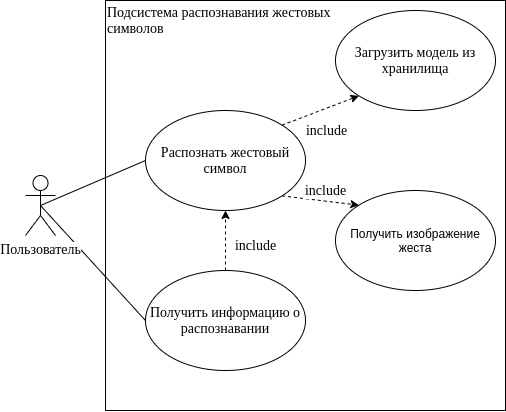
\includegraphics[width=0.6\textwidth]{inc/img/run_test}
	\caption{Функциональные возможности подсистемы распознавания жестовых символов}
	\label{impl:run_func}
\end{figure}

Каждый этап функционирования системы был реализован в виде обособленных модулей с унифицированными API и форматами данных. Функционал данного программного продукта может быть расширен путем добавления новых подсистем, а так же адаптирован под иные источники и форматы изображений жестовых символов.

\section{Построение нейронной сети}

В представлении Tensorflow нейронная сеть является графом потока данных, в котором данные в виде многомерного массива переходят в разные узлы, в процессе чего происходят все необходимые вычисления. Из-за данного подхода процесс описания нейронных сетей с использованием нативного Tensorflow затруднителен. Для упрощения построения моделей можно использовать библиотеку Keras, которая предоставляет простой и удобный способ создания моделей глубокого обучения. Данная библиотека имеет большую базу широко используемых типов слоев искусственных нейронных сетей, а так же предоставляет возможность описывать собственные слои через наследование базового класса Layer.

Алгоритм \ref{imp:init-model} описывает построение КНС. Для преобразования входного изображения в тенсор используется слой layers.Input.

\begin{minipage}{0.8\textwidth}
	\begin{algorithm}[H]
		\lstinputlisting[language=Python]{inc/src/model.py}
		\caption{Исходный код инициализации модели}
		\label{imp:init-model}
	\end{algorithm}
\end{minipage}

Капсулы первого капсульного слоя, как описано выше, представляют собой комбинацию нескольких сверточных слоев. В следствии этого, реализация данного слоя возможна стандартными слоями библиотеки Keras, как показано на алгоритме \ref{imp:prim}.

\begin{minipage}{0.8\textwidth}
	\begin{algorithm}[H]
		\lstinputlisting[language=Python]{inc/src/prim.py}
		\caption{Исходный код инициализации первого капсульного слоя}
		\label{imp:prim}
	\end{algorithm}
\end{minipage}


\begin{minipage}{0.8\textwidth}
	\begin{algorithm}[H]
		\lstinputlisting[language=Python]{inc/src/digit.py}
		\caption{Исходный код реализации динамической маршрутизации}
		\label{imp:digit}
	\end{algorithm}
\end{minipage}

Второй капсульный слой нельзя реализовать стандартными средствами пакета layers библиотеки Keras из-за необходимости самостоятельного описания алгоритма динамической маршрутизации. Для этого был описан класс, CapluleLayer, наследованный от класса layers.Layer. Реализация динамической маршрутизации представлена в алгоритме \ref{imp:digit}.

Итоговый граф изображен на рисунке \ref{impl:graph}.

\begin{figure}[!h]
	\centering
	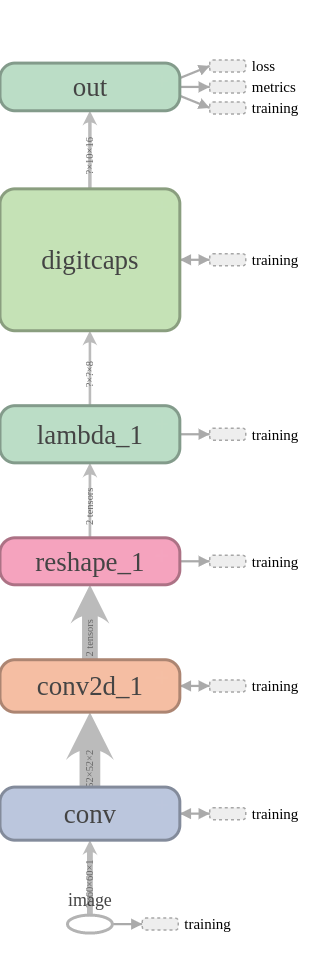
\includegraphics[width=0.3\textwidth]{inc/img/graph}
	\caption{Граф модели}
	\label{impl:graph}
\end{figure}

\section{Руководство пользователя}

\subsection*{Установка программного обеспечения}

Для запуска разработанного программного комплекса требуется установленный на ПК интерпретатор для Python 3. Все необходимые библиотеки указаны в файле requirements.txt, находящемся в корневом каталоге проекта. Средствами каталога программного обеспечения PyPI (Python Package Index) все зависимости устанавливаются выполнением одной команды в терминале:

\textbf{\$ pip3 install -r requirements.txt}

\subsection*{Подсистема обучения}

Обучение классификаторов происходит с помощи Jupyter Notebook -- интерактивной оболочки для языка Python. Данная технология позволяет объединяет код и вывод в окне одного документа, содержащего текст, математические уравнения и визуализации. Такой пошаговый подход обеспечивает быстрый, последовательный процесс разработки, поскольку вывод для каждого блока показывается сразу же.

Для работы и выполнения кода ноутбуков необходимо запустить сервер Jupiter, выполнив в корневом каталоге команду:

\textbf{\$ jupiter notebook}

После этого в стандартном браузере системы откроется сайт с URL http://localhost:8888/tree с файловым менеджером, открытым в корневом каталоге. Для запуска ноутбуков обучения нужно открыть в этом же окне любой файл из папки notebooks и нажать кнопку Run All. Результаты обучения сохраняются в папку data/название выборки/tensorboard.

\subsection*{Подсистема распознавания жестовых символов}

В подсистеме распознавания жестовых символов используется уже обученная нейронная сеть, файл с весовыми коэффициентами которой находится в папке data/название выборки/tensorboard. Для удобства пользователя программное обеспечение поставляется с набором уже обученных классификаторов. Для запуска программы используется команда 

\textbf{\$ python3 main.py}

После запуска программы появляется главное окно (рисунок \ref{impl:main_start}).

\begin{figure}[!h]
	\centering
	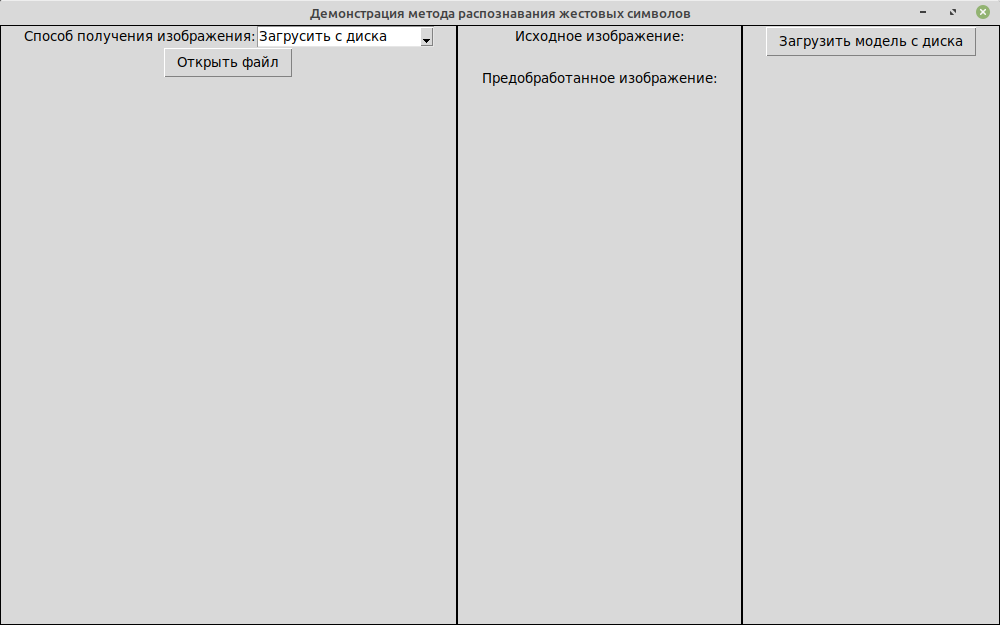
\includegraphics[width=0.7\textwidth]{inc/img/main_start}
	\caption{Окно программы после запуска}
	\label{impl:main_start}
\end{figure}

Визуально область окна разделена на 3 зоны:
\begin{itemize}
	\item Зона загрузки данных. Управляет методом получения изображения. Изначально указан метод <<Загрузить с диска>>, отображающий кнопку <<Открыть файл>>, при нажатии которого открывается диалоговое окно выбора файла изображения. При переключении на метод <<Снять с web-камеры>> открывается окно с демонстрацией видео-потока с web-камеры и кнопкой <<Сделать снимок>> (рисунок \ref{impl:main_webcam}).
	
	\begin{figure}[!h]
		\centering
		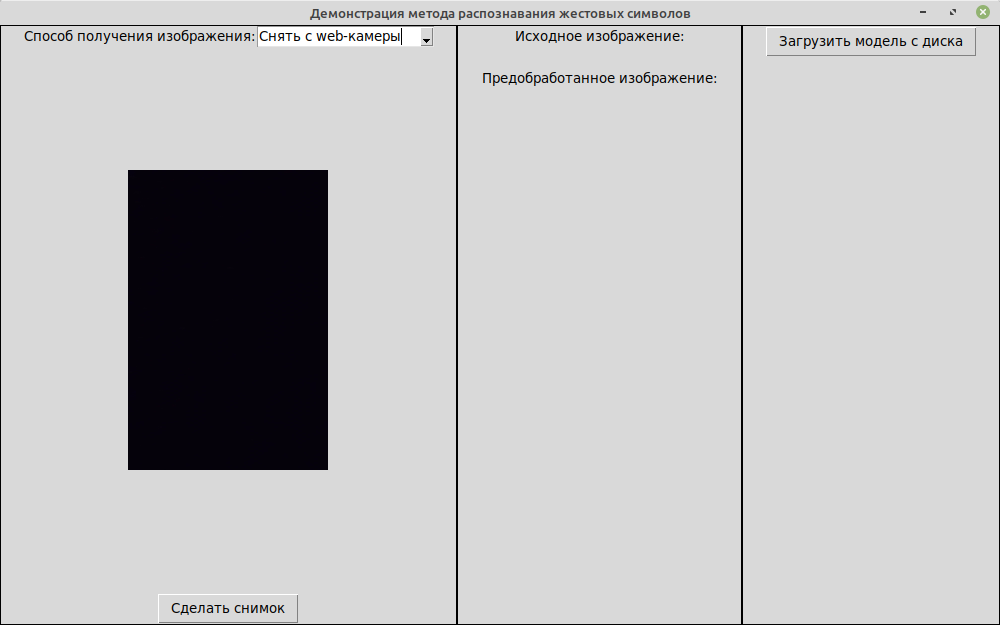
\includegraphics[width=0.7\textwidth]{inc/img/main_webcam}
		\caption{Окно программы в режиме получения изображения с web-камеры}
		\label{impl:main_webcam}
	\end{figure}

	\item Зона предварительно обработки. После получения входных данных отображает два изображения: оригинальное и результат предобработки (рисунок \ref{impl:main}).
	
	\begin{figure}[!h]
		\centering
		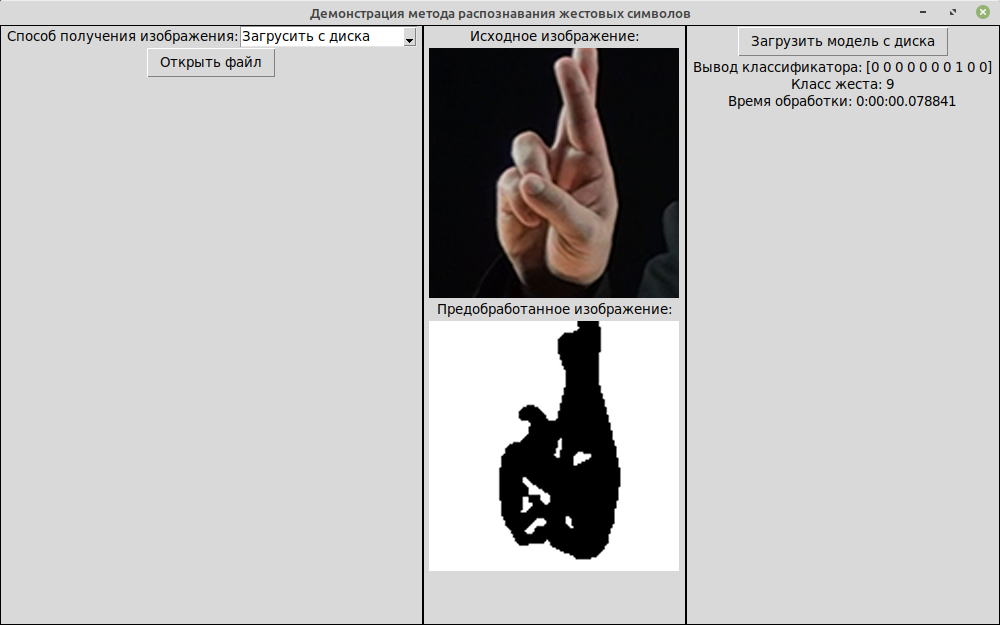
\includegraphics[width=0.6\textwidth]{inc/img/main}
		\caption{Окно программы после классификации}
		\label{impl:main}
	\end{figure}

	\item Зона классификации. Кнопка <<Загрузить модель с диска>> открывает диалоговое окно выбора файла весовых коэффициентов КНС. Ниже отображаются результаты классификации: исходный вывод модели, интерпретированный результат классификации и время полной обработки изображения.
\end{itemize}

\section{Вывод}

Была разработана архитектура программного комплекса для демонстрации работы метода классификации жестовых символов. Процесс обучения и эксплуатации системы выделены в отдельные подсистемы для упрощения разработки. Проведена декомпозиция подсистем на модули, позволяющие расширять функционал программного продукта путем добавления новых модулей.

На основе спроектированной архитектуры был разработан программный комплекс на языке Python с использованием библиотек OpenCV, scikit-learn, NumPy, Tensorflow, Keras и Tkinter.

Продукт был разработан на ЭВМ со следующими характеристиками:

\begin{itemize}
	\item Процессор: Intel© Core™ i5-8250U.
	\item Тактовая частота: 1.60ГГц $\times$ 4
	\item Объем оперативной памяти: 8 Гб.
	\item Графическая карта: Intel Corporation UHD Graphics 620.
	\item Операционная система: Linux Mint 19.3 Cinnamon.
	\item Версия ядра Linux: 5.3.0-53-generic.
\end{itemize}
\chapter{Экспериментальный раздел}
\label{cha:research}

В рамках дипломного проекта был ряд экспериментов, направленных на исследование построенного метода распознавания жестовых интерфейсов. Целью проведенных исследований является выяснение зависимости качества классификации от этапа предобработки и количества итераций в алгоритме динамической маршрутизации.

В качестве входных данных использовались изображения жестов, выполненные как мужчинами, так и женщинами различной национальности.

\section{Описание тестовых данных}

Для проведения вычислительных экспериментов использовались следующие наборы данных:

\begin{itemize}
	\item ASL Finger Spelling Dataset -- набор изображений дактилей американского жестового языка. Использовался для оценки качества распознавания в описанных ранее методах \cite{Karn,Starner,Garcia}. На основании результатов данной выборке делается вывод о качестве построенного метода относительно конкурентов. Данный датасет состоит из двух частей: изображений 24 дактилических жестов (в данную выборку не входят буквы <<j>> и <<z>>, так как являются динамическими) и карт глубин. В данной работе использовалась первая часть, которая состоит из 65000 изображений с непостоянным размером в цветовом пространстве RGB. Жесты демонстрируются пятью разными людьми.
	\item RSL by Oleg Potkin -- набор данных русского дактиля. Содержит 1042 RGB изображения размером 128$\times$128 пикселей. Разделен на 10 классов-букв: <<а>>, <<б>>, <<в>>, <<г>>, <<е>>, <<и>>, <<о>>, <<п>>, <<с>>.
	\item Numbers -- набор данных c изображением жестов цифр. Состоит из из 1125 RGB изображений.
\end{itemize}

\section{Формальная модель и описание условий исследования}

Для выявления зависимости качества распознавания от количества итераций в алгоритме динамической маршрутизации в рамках исследования для одного набора данных строились модели для двух, трех, четырех, пяти, шести и семи итераций. Каждая модель обучалась на предобработанных и оригинальных наборах данных.

Для проведения вычислительных экспериментов была разработана формальная модель, представленная на рисунке \ref{res:research}.

\begin{figure}
	\centering
	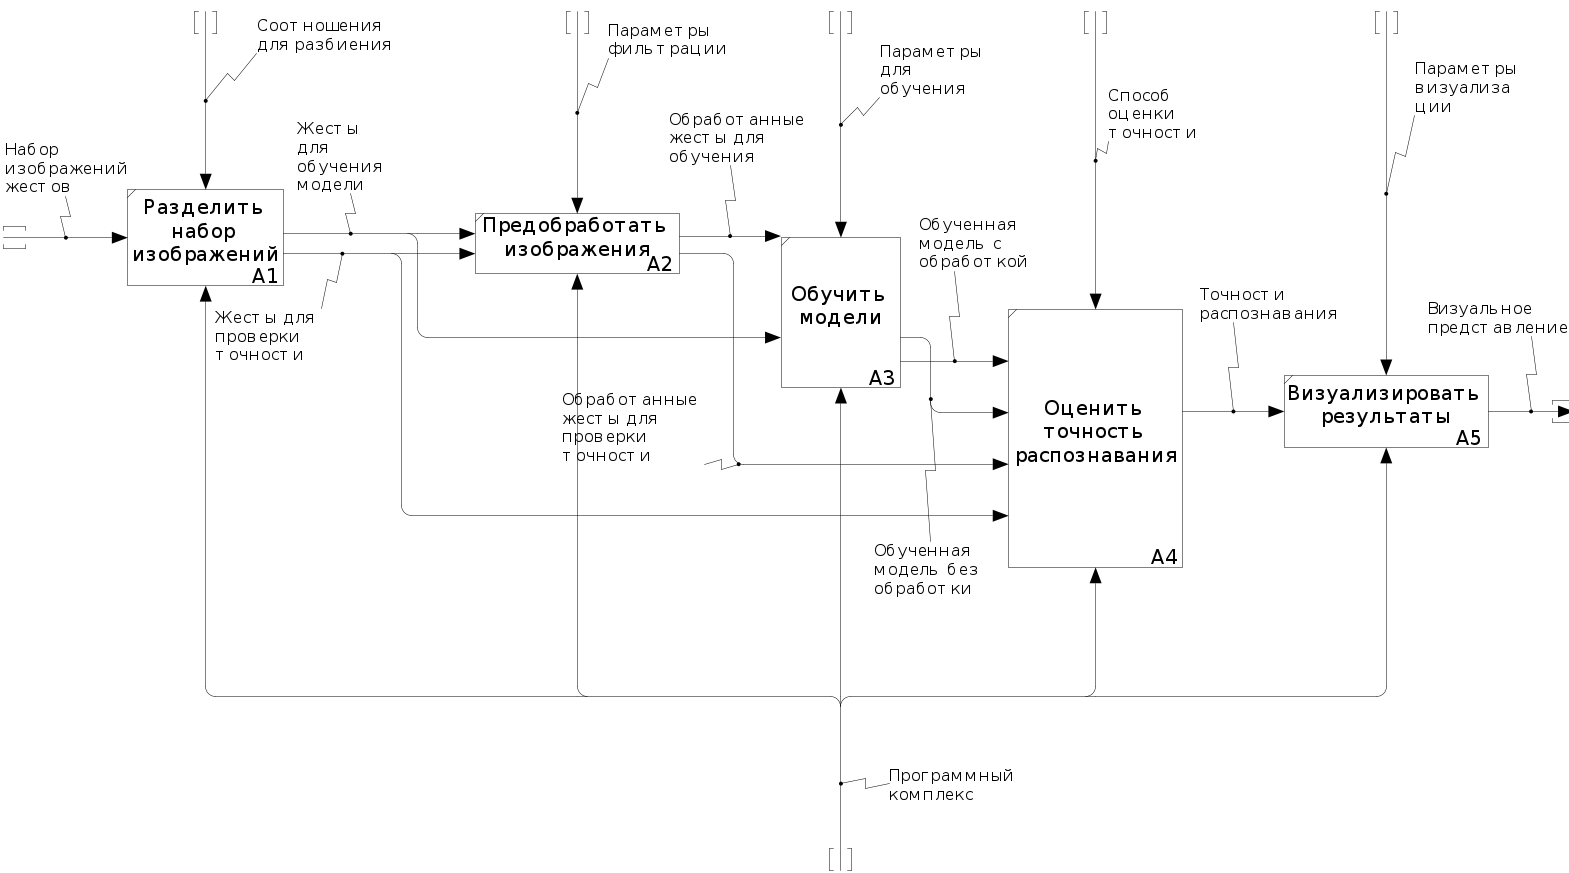
\includegraphics[width=\textwidth]{inc/img/research}
	\caption{Формальная модель эксперимента}
	\label{res:research}
\end{figure}

В качестве метрики качества распознавания метода используется вероятность корректной классификации жестового символа (формула \ref{res:acc}).

\begin{equation}
\label{res:acc}
\text{Точность} = \frac{\text{Верные классификации}}{\text{Ложные классификации} + \text{Верные классификации}}
\end{equation}

Каждый набор изображений был разделен в соотношении 20\% для валидации, 64\% для обучения и 16\% для тестирования. 

Исследования проводились с использованием платформы Google Colaboratory, предоставляющая бесплатное выполнение файлов ipython notebook с использованием GPU и TPU. В рамках одной сессии предоставляется 25,51 Гб ОЗУ и 68,40 дискового пространства.

\section{Результаты исследований}

Для оптимальной настройки описанного метода были проведены вычислительные эксперименты с целью определения зависимости точности распознавания от числа итераций динамичесой маршрутизации. Для выяснения влияния этапа предобработки на качество работы классификатора данные вычисления проводились для обработанных и исходных наборов изображений. Результаты экспериментов были обобщены и виде графиков, представленных на рисунках \ref{res:asl}, \ref{res:rsl_oleg} и \ref{res:number}

\begin{figure}[!h]
	\centering
	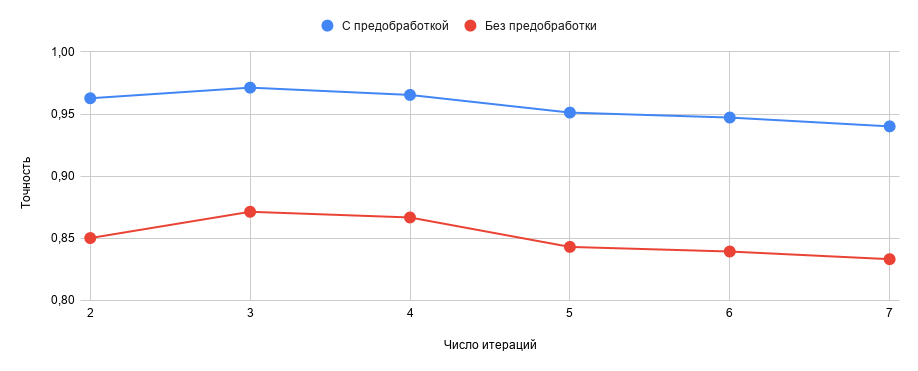
\includegraphics[width=0.9\textwidth]{inc/img/asl}
	\caption{Зависимость точности распознавания от предобработки входных данных и числе итераций на датасете ASL Finger Spelling Dataset}
	\label{res:asl}
\end{figure}

\begin{figure}[!h]
	\centering
	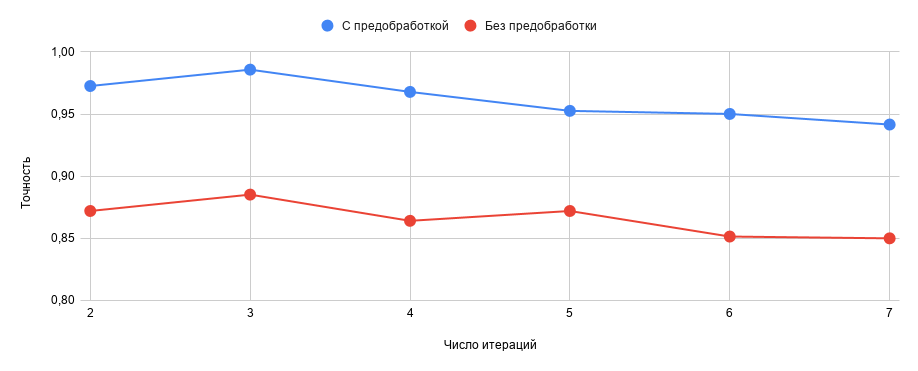
\includegraphics[width=0.9\textwidth]{inc/img/rsl_oleg}
	\caption{Зависимость точности распознавания от предобработки входных данных и числе итераций на датасете RSL by Oleg Potkin}
	\label{res:rsl_oleg}
\end{figure}

\begin{figure}[!h]
	\centering
	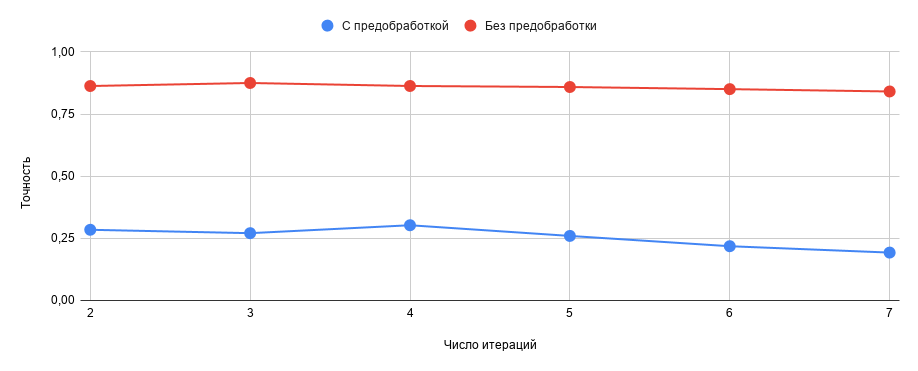
\includegraphics[width=0.9\textwidth]{inc/img/rsl_hse}
	\caption{Зависимость точности распознавания от предобработки входных данных и числе итераций на датасете Numbers}
	\label{res:number}
\end{figure}

Исследование показало, что предобработка изображений позволяет увеличить точность распознавания в среднем на 10-15 \%, как видно на рисунках \ref{res:asl} и \ref{res:rsl_oleg}. С другой стороны, есть вероятность получения зашумленных предобработанных изображений, следствием чего является потеря работоспособности классификатора (рисунок \ref{res:number}). Пример зашумленного предобработанного изображения представлен на рисунке \ref{res:bad_preproc}.

\begin{figure}[ht!]
	\begin{minipage}[h]{0.49\linewidth}
		\center{
\includegraphics[width=0.5\linewidth]{inc/img/preprocessing/bad_orig} \\ а)}
	\end{minipage}
	\hfill
	\begin{minipage}[h]{0.49\linewidth}
		\center{
\includegraphics[width=0.5\linewidth]{inc/img/preprocessing/bad_res} \\ б)}
	\end{minipage}
	\caption{Результат предобработки изображения из датасета Number с зашумлением: а) исходное изображение; б) предобработанное изображение}
	\label{res:bad_preproc}
\end{figure}

Наибольшая точность распознавания достигается при трех итерациях алгоритма маршрутизации, как видно на рисунках \ref{res:asl} и \ref{res:rsl_oleg}.

\section{Анализ полученных результатов}

В связи с тем, что набор ASL  Finger Spelling Dataset использовался в ряде дру­гих исследований в области распознавания жестовых символов, опуб­ликованных в последние годы, стало возможным сравнить результаты распознавания предложенного метода с аналогичными методами.

Точность распознавания для других методов представлена на ри­сункe \ref{res:compare}.

\begin{figure}[!h]
	\centering
	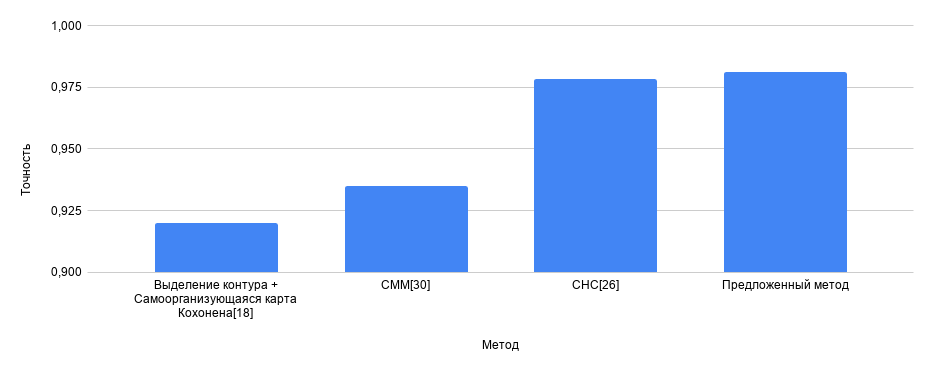
\includegraphics[width=\textwidth]{inc/img/compare}
	\caption{Сравнение точности распознавания известных методов}
	\label{res:compare}
\end{figure}

Полученные результаты показывают, что разработанный метод на 3\% позволяет повысить точность распознавания жестовых символов.


\backmatter %% Здесь заканчивается нумерованная часть документа и начинаются ссылки и
            %% заключение

\Conclusion % заключение к отчёту

В результате проделанной работы были решены следующие задачи:

\begin{itemize}
	\item был проведен анализ предметной области;
	\item были проанализированы существующие решения;
	\item на основе полученных во время анализа данных был разработан собственный метод выделения голосовой составляющей из монофонического аудио сигнала;
	\item предложенный метод был реализован в программном продукте.
\end{itemize}

В результате тестирования и эксперимента было установлено, что разработанный метод:

\begin{itemize}
	\item для вокала имеет примерно те же показатели метрик, что и метод FASST, при этом имея в среднем в два раза меньший разброс, для аккомпанемента же средние значения метрик в среднем на 60\% лучше, имея примерно те же значения разброса;
	\item для вокала значение метрик в среднем на 80\% лучше, чем у метода ГНС, при этом дисперсия в среднем в два раза меньше. Для аккомпанемента значение средних метрик приблизительно одинаков, но значение дисперсии у разработанного метода на 30\% меньше;
	\item для вокала значение метрик в среднем в 2,5 раза уступают методу СНС, при этом дисперсия в среднем в 2 раза лучше. Для аккомпанемента метрики примерно одинаковые, но разброс у разработанного метода в среднем в 2 раза больше, чем у метода СНС.
\end{itemize}

В результате тестирования и эксплуатации разработанного ПО заменен основной недостаток -- наличие примесей из соседних источников в выделяемом сигнале

Развитие разработанного метода можно осуществлять по следующим направлениям:

\begin{itemize}
	\item увеличение качества выделения переработкой архитектуры сети;
	\item определение источников, участвовавших в записи исходного сигнала.
\end{itemize}

%%% Local Variables: 
%%% mode: latex
%%% TeX-master: "rpz"
%%% End: 


% % Список литературы при помощи BibTeX
% Юзать так:
%
% pdflatex rpz
% bibtex rpz
% pdflatex rpz

\bibliographystyle{gost780u}

\bibliography{rpz}

%%% Local Variables: 
%%% mode: latex
%%% TeX-master: "rpz"
%%% End: 


%\appendix   % Тут идут приложения

\chapter{ПРИЛОЖЕНИЕ А}
\label{cha:appendix1}

пфывафываФЫАФА ФЫВФЫВФЫВ пфывафываФЫАФА ФЫВФЫВФЫВ пфывафываФЫАФА ФЫВФЫВФЫВ пфывафываФЫАФА ФЫВФЫВФЫВ пфывафываФЫАФА ФЫВФЫВФЫВ пфывафываФЫАФА ФЫВФЫВФЫВ пфывафываФЫАФА ФЫВФЫВФЫВ пфывафываФЫАФА ФЫВФЫВФЫВ пфывафываФЫАФА ФЫВФЫВФЫВ пфывафываФЫАФА ФЫВФЫВФЫВ пфывафываФЫАФА ФЫВФЫВФЫВ пфывафываФЫАФА ФЫВФЫВФЫВ пфывафываФЫАФА ФЫВФЫВФЫВ пфывафываФЫАФА ФЫВФЫВФЫВ пфывафываФЫАФА ФЫВФЫВФЫВ пфывафываФЫАФА ФЫВФЫВФЫВ пфывафываФЫАФА ФЫВФЫВФЫВ пфывафываФЫАФА ФЫВФЫВФЫВ пфывафываФЫАФА ФЫВФЫВФЫВ пфывафываФЫАФА ФЫВФЫВФЫВ пфывафываФЫАФА ФЫВФЫВФЫВ пфывафываФЫАФА ФЫВФЫВФЫВ пфывафываФЫАФА ФЫВФЫВФЫВ пфывафываФЫАФА ФЫВФЫВФЫВ пфывафываФЫАФА ФЫВФЫВФЫВ пфывафываФЫАФА ФЫВФЫВФЫВ пфывафываФЫАФА ФЫВФЫВФЫВ пфывафываФЫАФА ФЫВФЫВФЫВ пфывафываФЫАФА ФЫВФЫВФЫВ пфывафываФЫАФА ФЫВФЫВФЫВ пфывафываФЫАФА ФЫВФЫВФЫВ пфывафываФЫАФА ФЫВФЫВФЫВ пфывафываФЫАФА ФЫВФЫВФЫВ пфывафываФЫАФА ФЫВФЫВФЫВ пфывафываФЫАФА ФЫВФЫВФЫВ пфывафываФЫАФА ФЫВФЫВФЫВ пфывафываФЫАФА ФЫВФЫВФЫВ пфывафываФЫАФА ФЫВФЫВФЫВ пфывафываФЫАФА ФЫВФЫВФЫВ пфывафываФЫАФА ФЫВФЫВФЫВ пфывафываФЫАФА ФЫВФЫВФЫВ пфывафываФЫАФА ФЫВФЫВФЫВ пфывафываФЫАФА ФЫВФЫВФЫВ пфывафываФЫАФА ФЫВФЫВФЫВ пфывафываФЫАФА ФЫВФЫВФЫВ пфывафываФЫАФА ФЫВФЫВФЫВ пфывафываФЫАФА ФЫВФЫВФЫВ пфывафываФЫАФА ФЫВФЫВФЫВ пфывафываФЫАФА ФЫВФЫВФЫВ пфывафываФЫАФА ФЫВФЫВФЫВ пфывафываФЫАФА ФЫВФЫВФЫВ пфывафываФЫАФА ФЫВФЫВФЫВ пфывафываФЫАФА ФЫВФЫВФЫВ 

%%% Local Variables: 
%%% mode: latex
%%% TeX-master: "rpz"
%%% End: 

%\chapter{Еще картинки}
\label{cha:appendix2}

\begin{figure}
\centering
\caption{Еще одна картинка, ничем не лучше предыдущей. Но надо же как-то заполнить место.}
\end{figure}

%%% Local Variables: 
%%% mode: latex
%%% TeX-master: "rpz"
%%% End: 


\end{document}

%%% Local Variables:
%%% mode: latex
%%% TeX-master: t
%%% End:
